\section{对话实例}

% \begin{frame}
% \frametitle{概述}
% \begin{itemize}
%     \item 本节展示 DeepSeek R1 模型在解决数学问题上的能力。
%     \item 包含 2024 AIME I Problem 4 和 2025 考研数学一 T18 两道例题。
% \end{itemize}
% \end{frame}

\subsection{2024 AIME I Problems/Problem 4}

\begin{frame}
    \frametitle{2024 AIME I Problem 4}
    % \textbf{题目描述}
    \begin{figure}
        \centering
        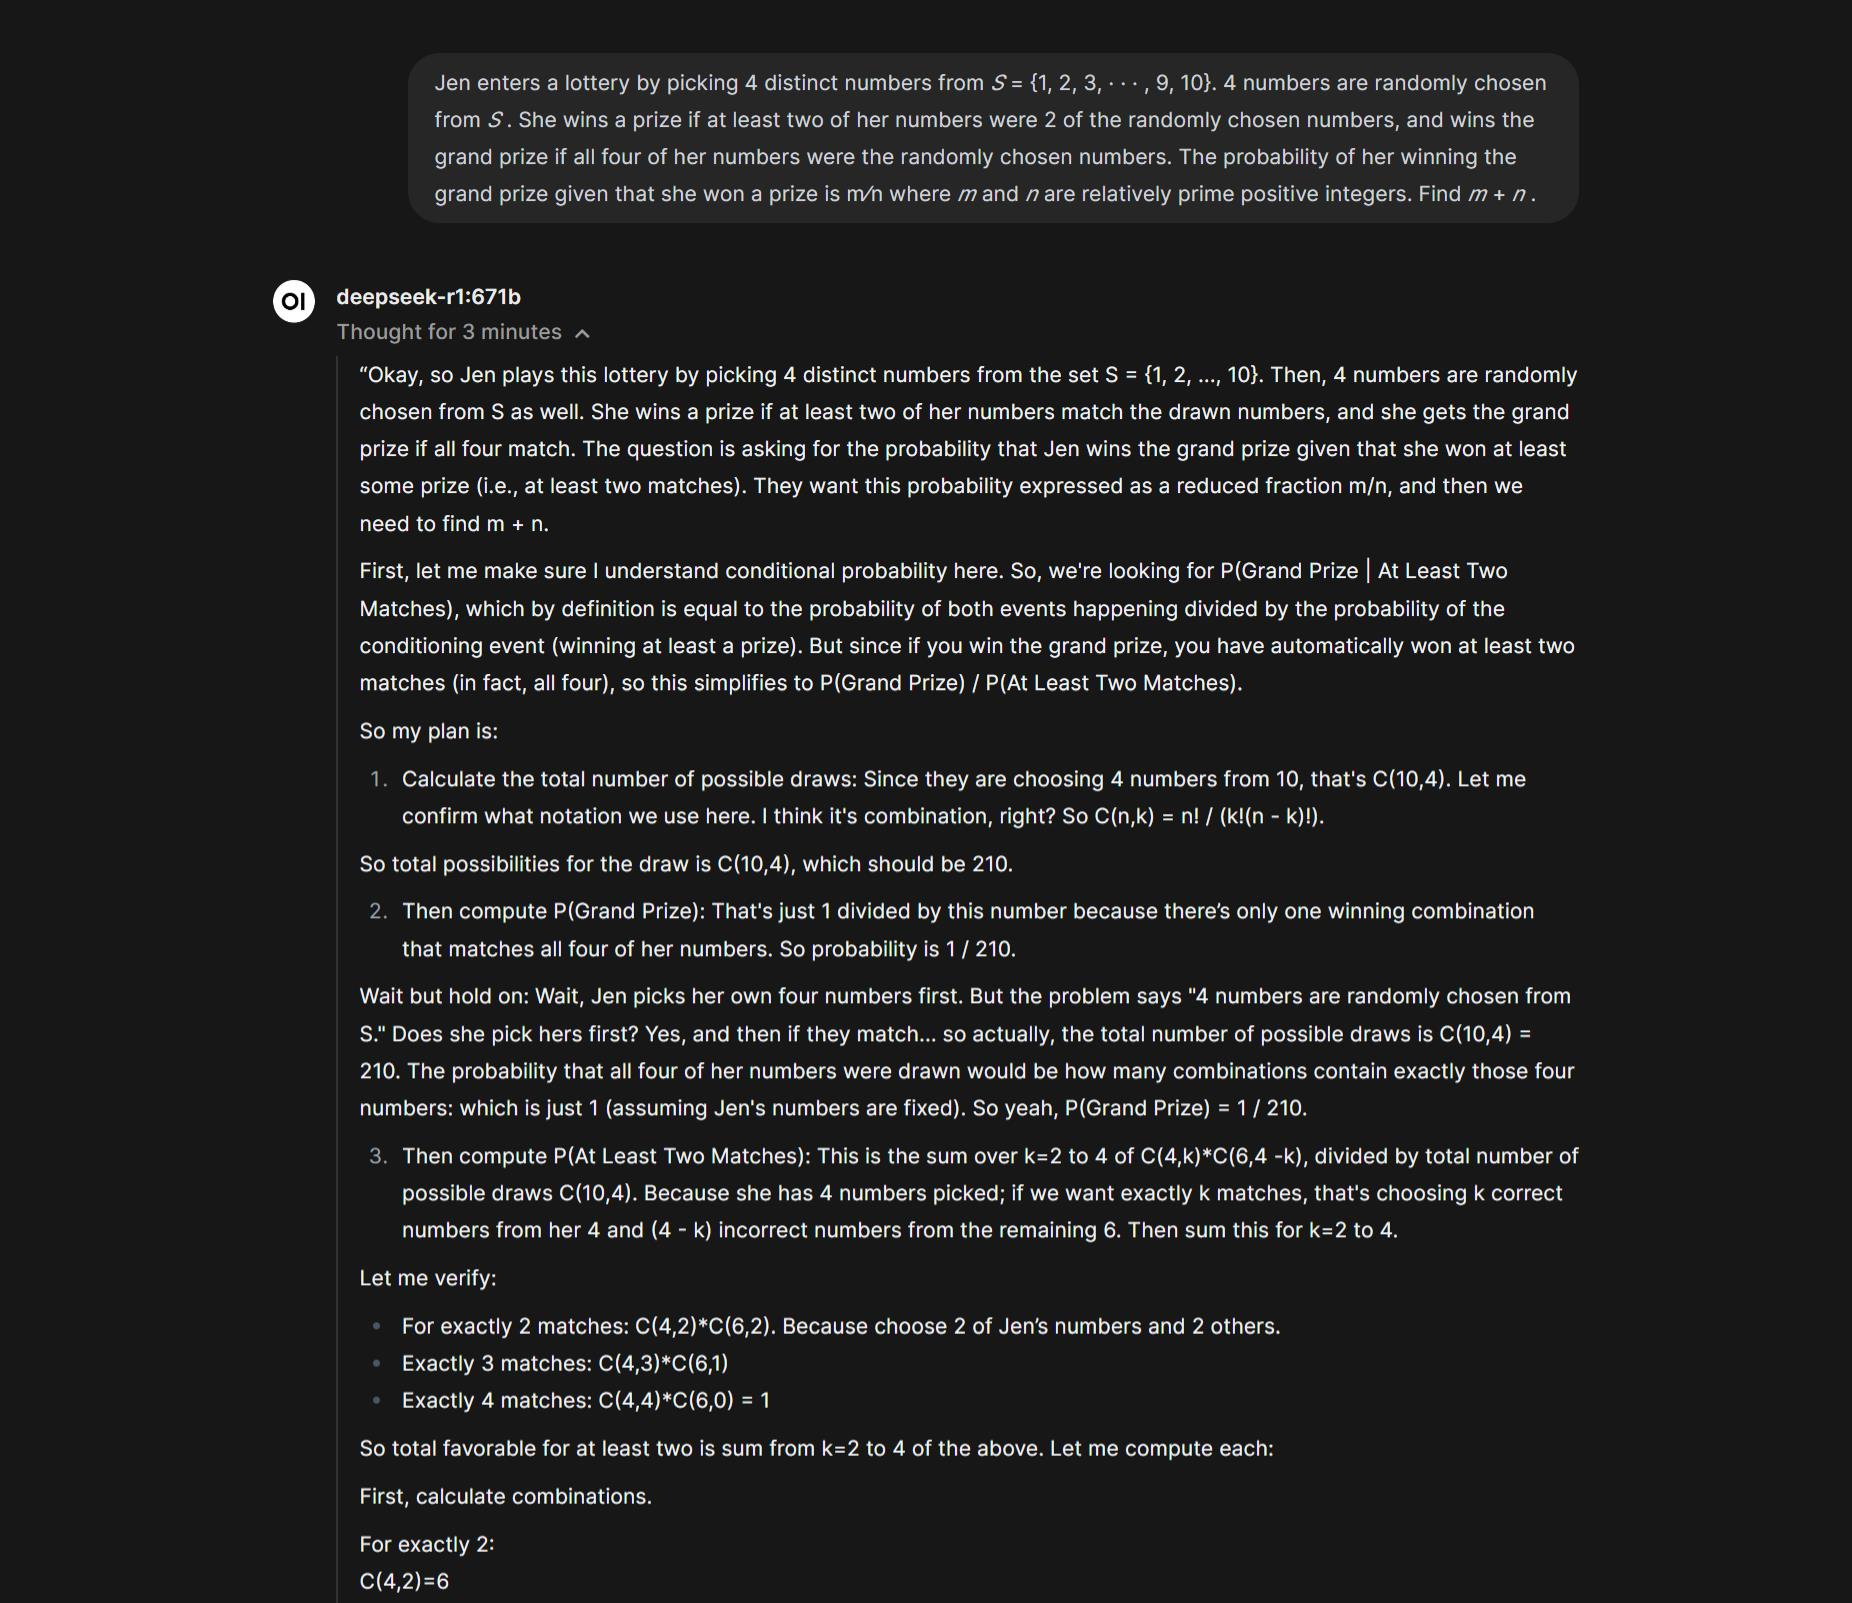
\includegraphics[width=0.55\textwidth]{./pic/2.png} % 替换为你的图片路径
        % \caption{2024 AIME I Problem 4 题目描述 (请替换为实际图片路径)}
        \label{fig:aime_problem_1}
    \end{figure}
    % \textit{图片来源: \url{https://raw.githubusercontent.com/Lanthanum1/my_images/main/img/202502112140491.png}} % 图片来源注释
\end{frame}

\begin{frame}
    \frametitle{2024 AIME I Problem 4 (续)}
    % \textbf{模型解答 (1)}
    \begin{figure}
        \centering
        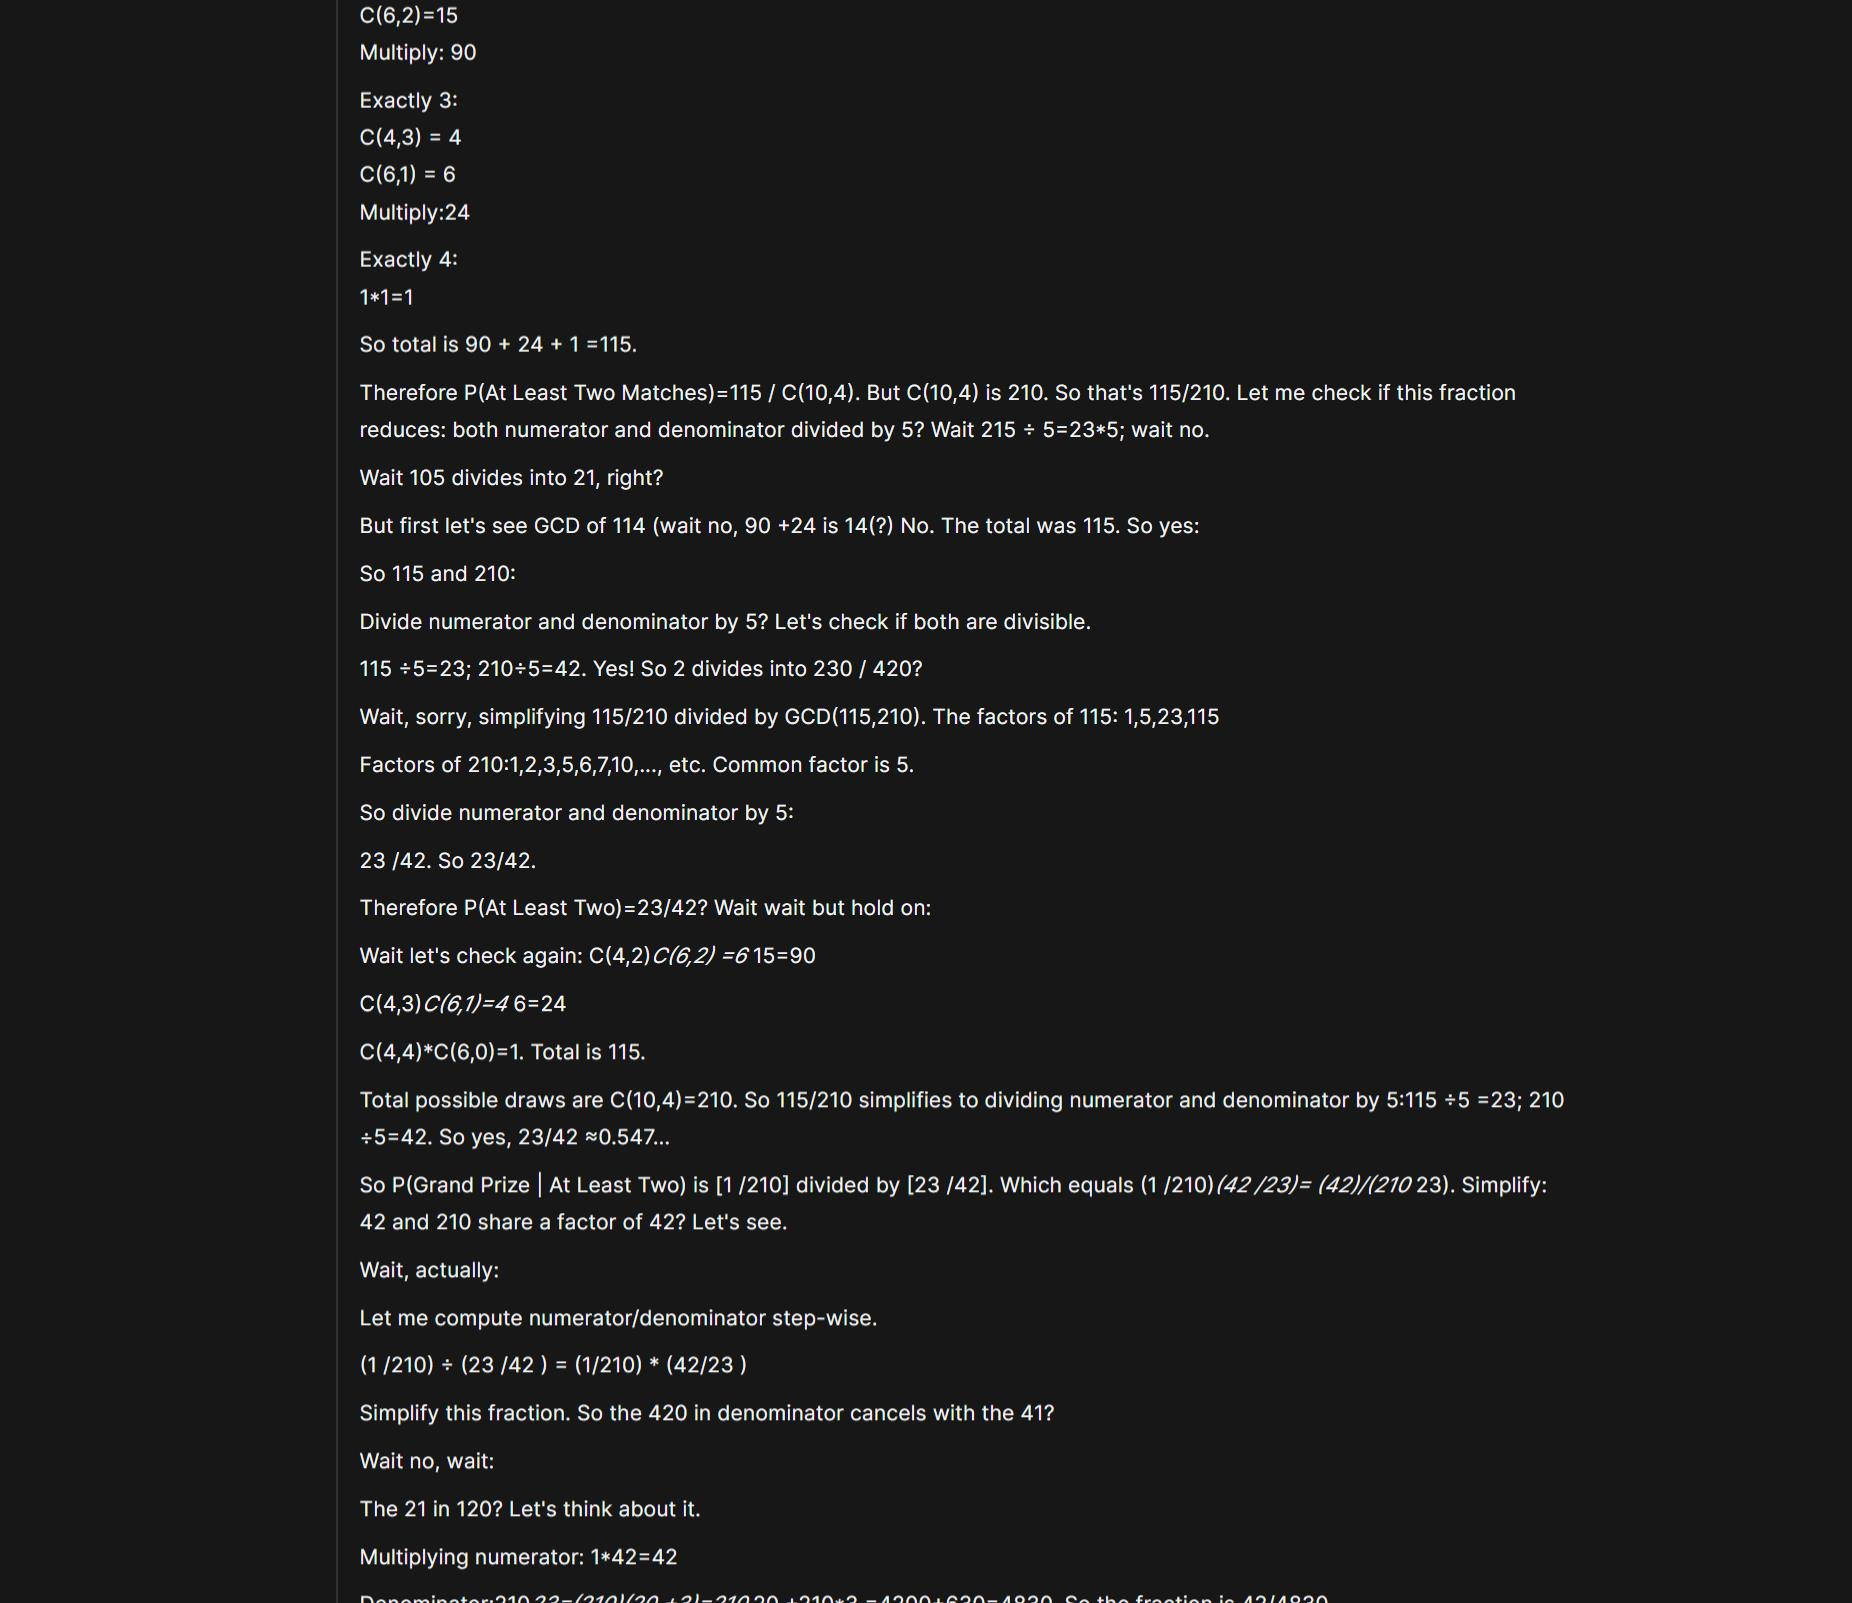
\includegraphics[width=0.55\textwidth]{./pic/3.png} % 替换为你的图片路径
        % \caption{DeepSeek R1 对 2024 AIME I Problem 4 的解答 (1) (请替换为实际图片路径)}
        \label{fig:aime_solution_1}
    \end{figure}
    % \textit{图片来源: \url{https://raw.githubusercontent.com/Lanthanum1/my_images/main/img/202502112140334.png}} % 图片来源注释
\end{frame}

\begin{frame}
    \frametitle{2024 AIME I Problem 4 (续)}
    % \textbf{模型解答 (2)}
    \begin{figure}
        \centering
        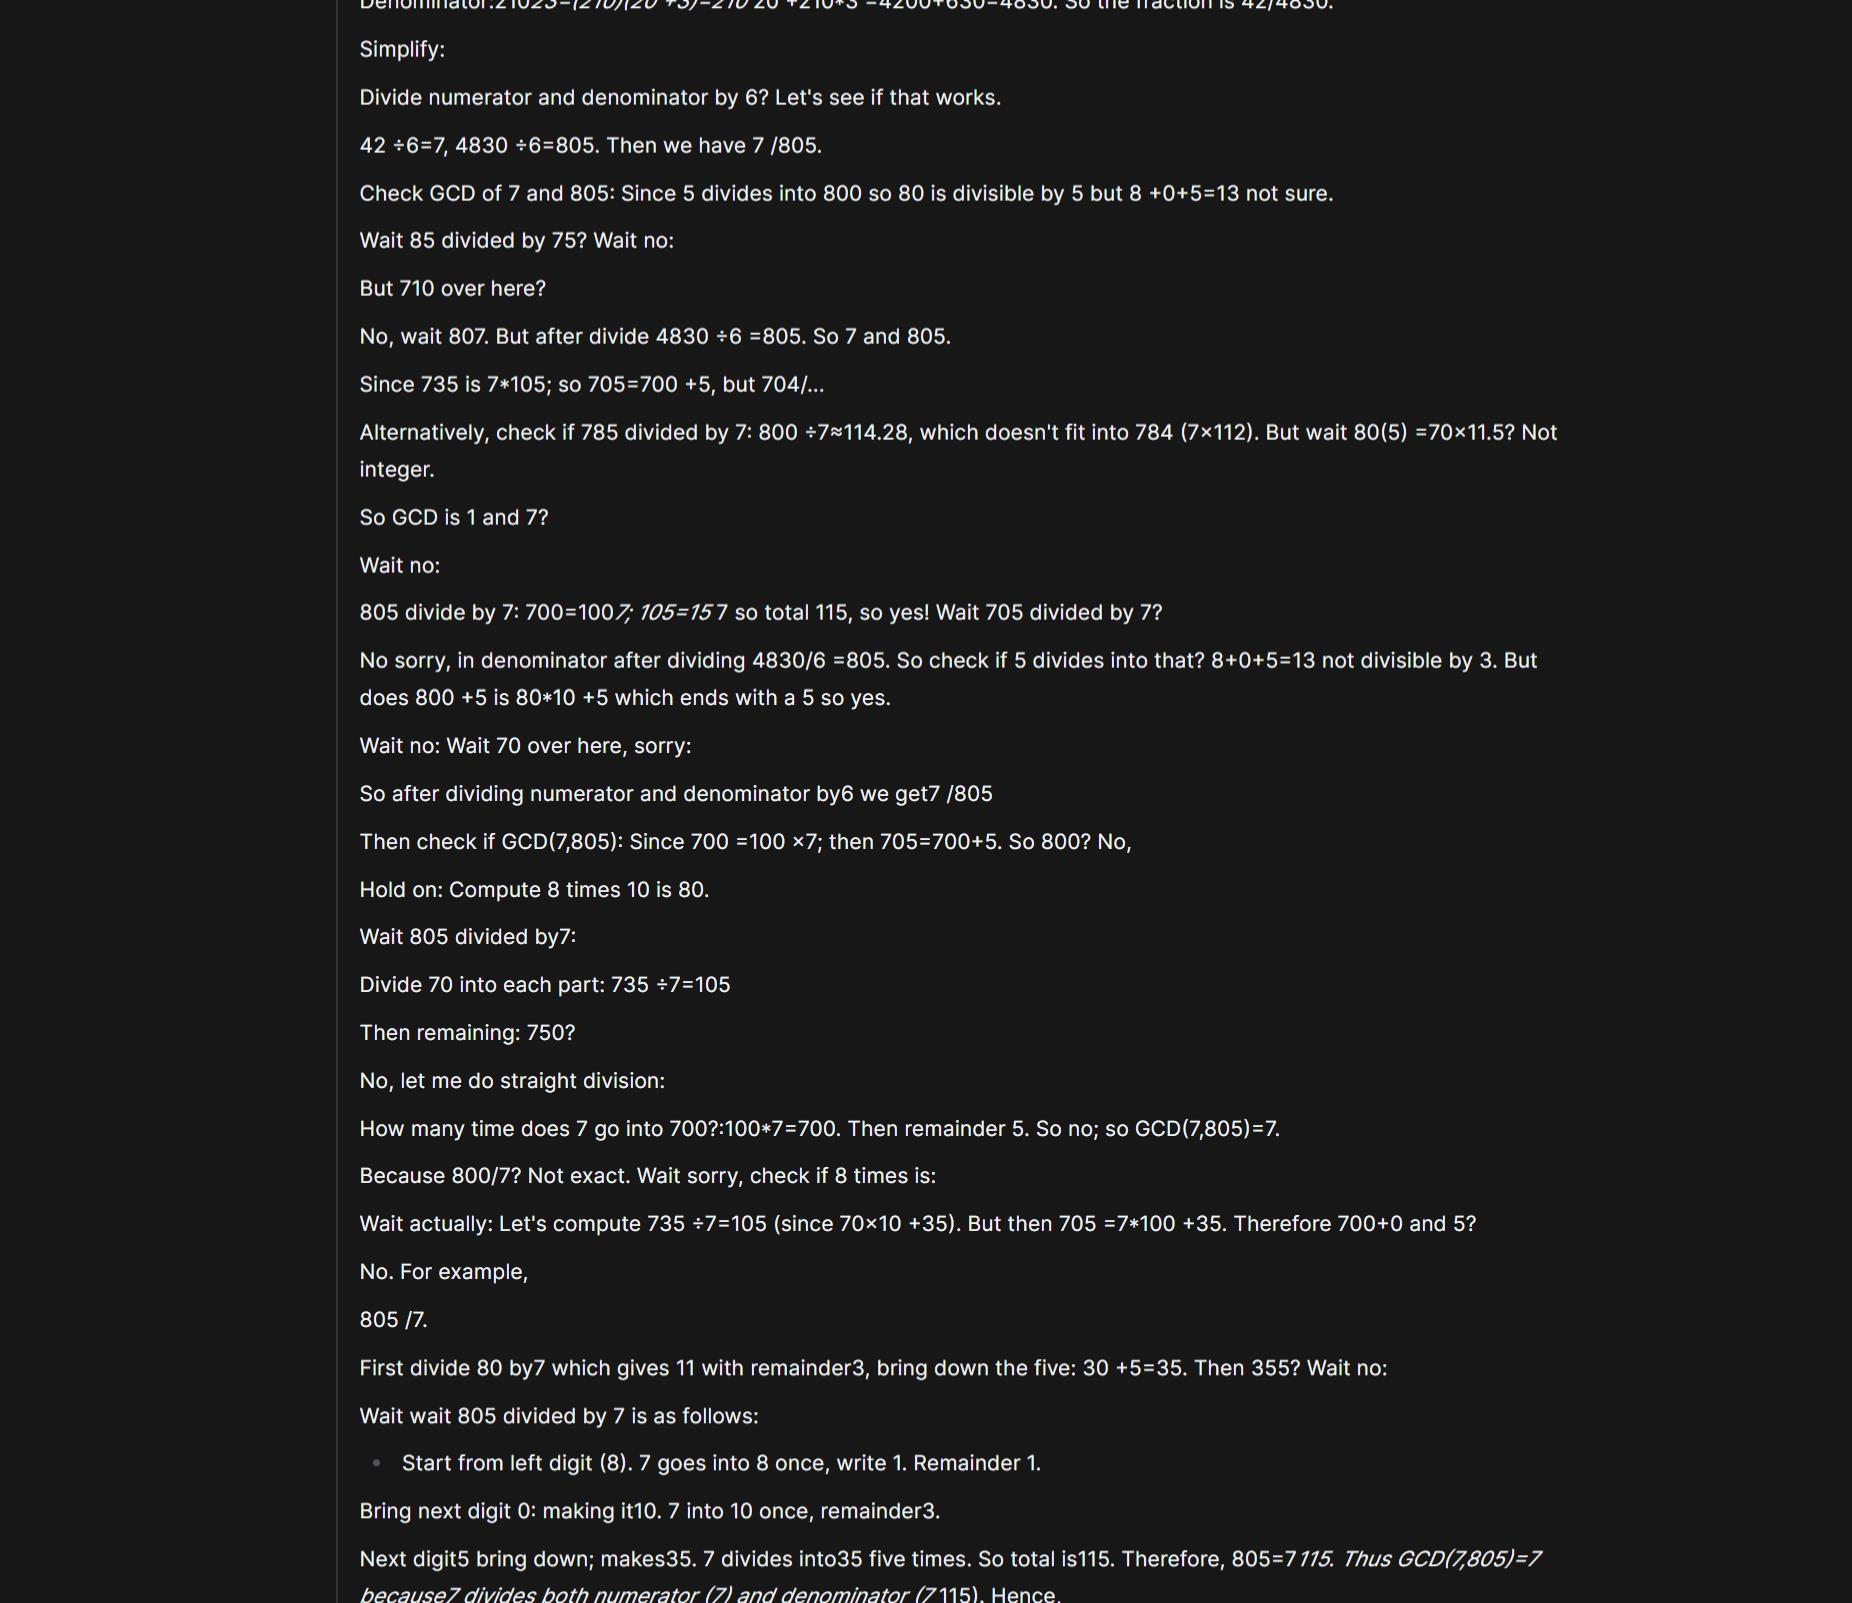
\includegraphics[width=0.55\textwidth]{./pic/4.png} % 替换为你的图片路径
        % \caption{DeepSeek R1 对 2024 AIME I Problem 4 的解答 (2) (请替换为实际图片路径)}
        \label{fig:aime_solution_2}
    \end{figure}
    % \textit{图片来源: \url{https://raw.githubusercontent.com/Lanthanum1/my_images/main/img/202502112143713.png}} % 图片来源注释
\end{frame}

\begin{frame}
    \frametitle{2024 AIME I Problem 4 (续)}
    % \textbf{模型解答 (3)}
    \begin{figure}
        \centering
        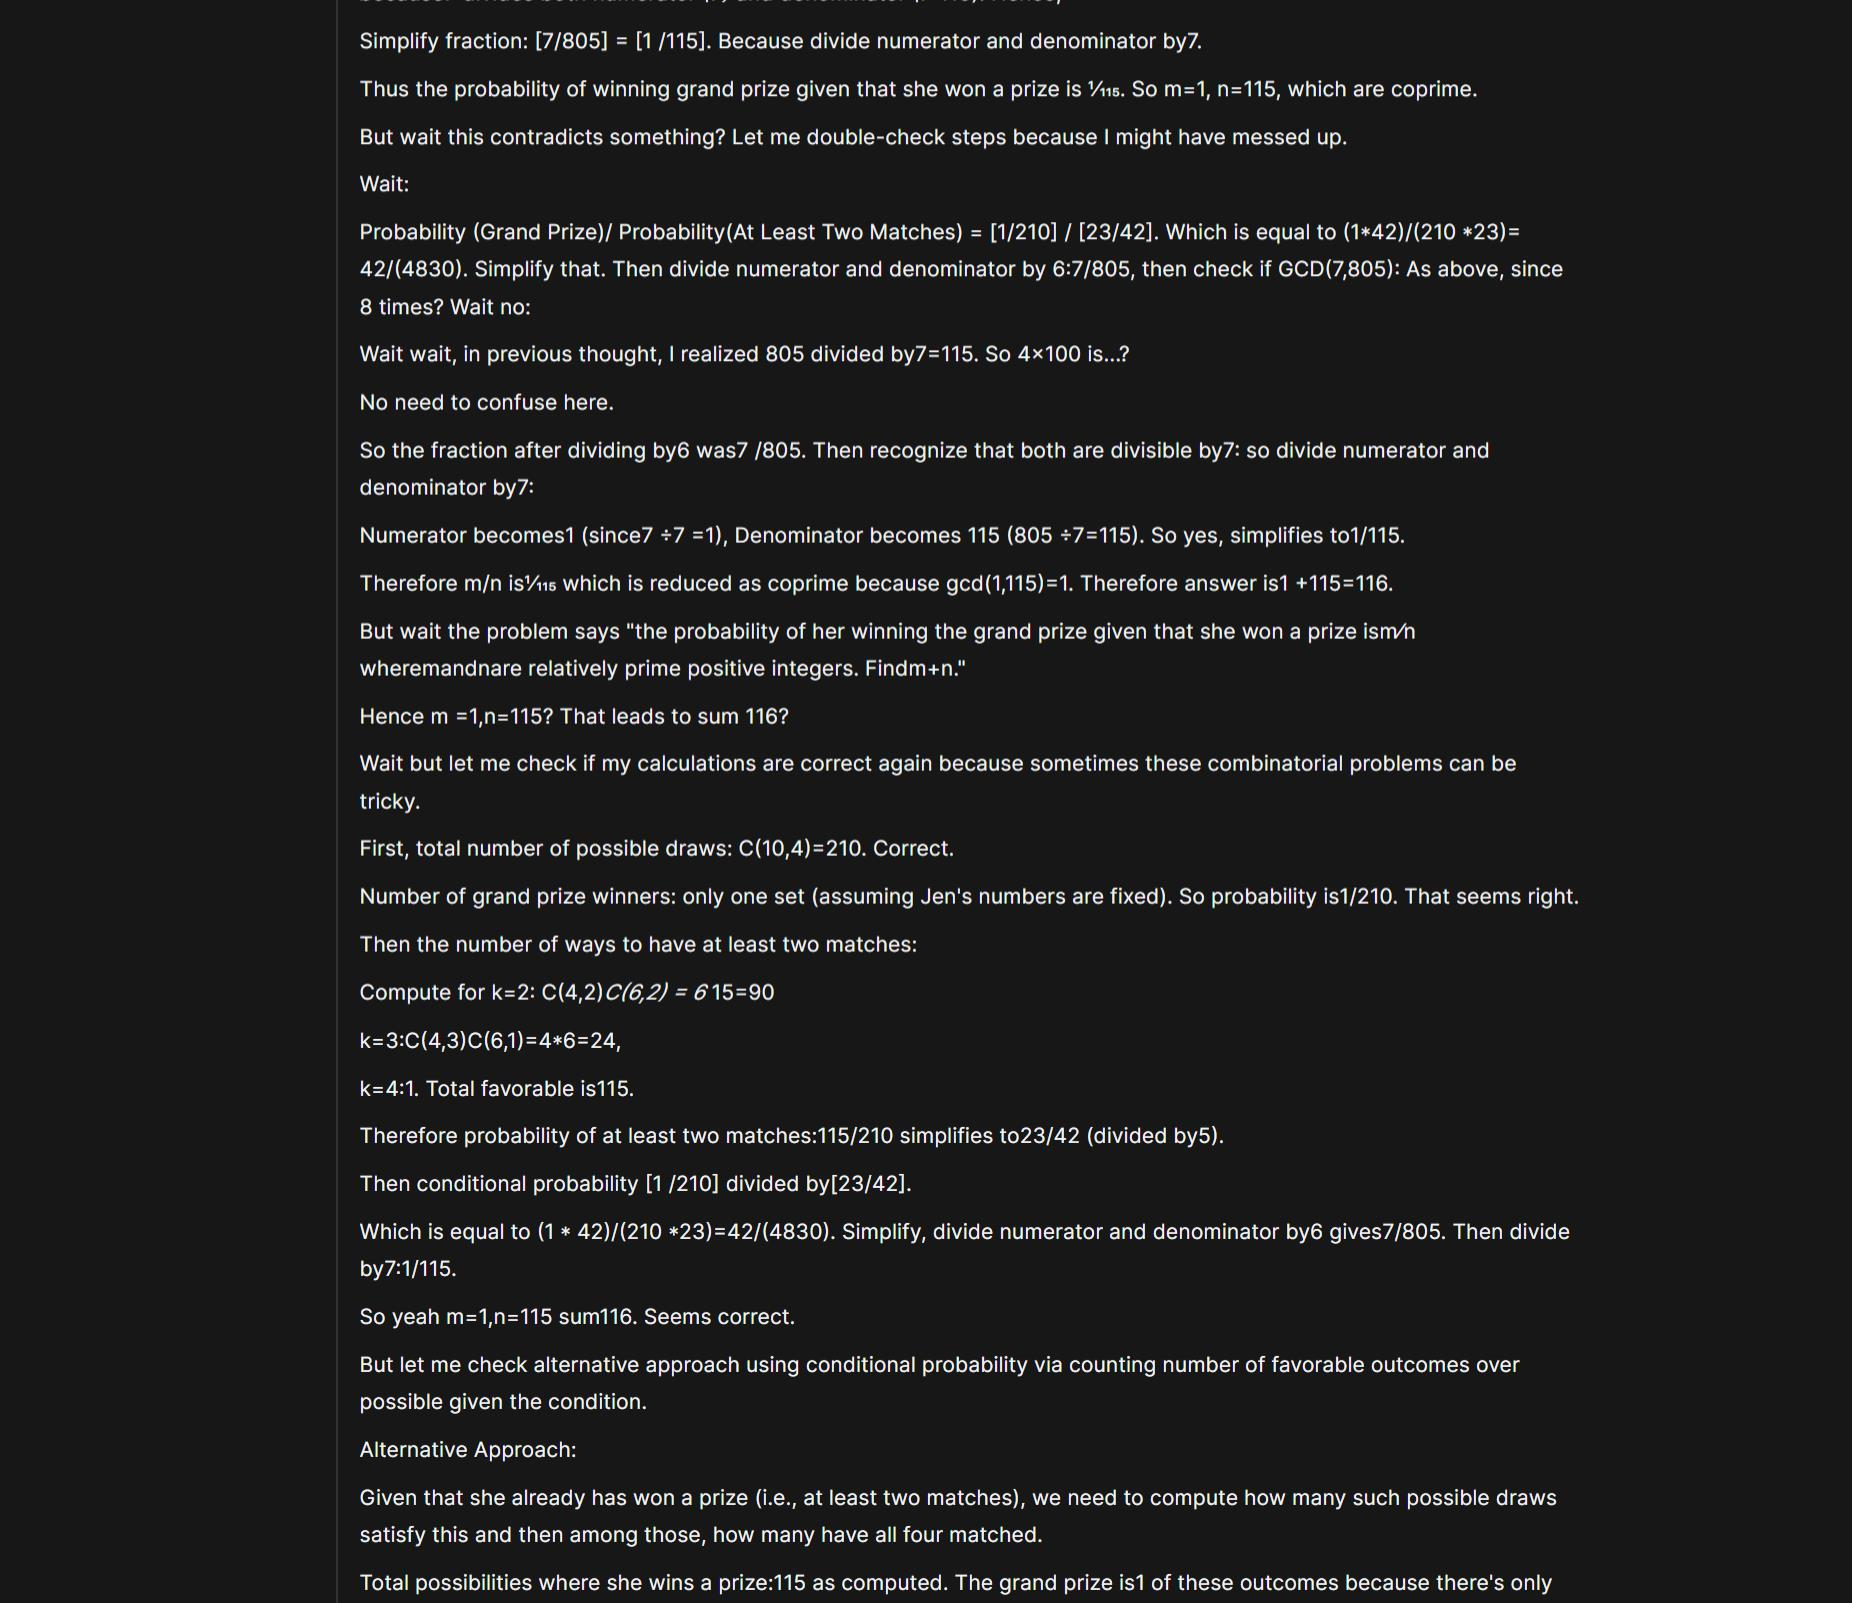
\includegraphics[width=0.55\textwidth]{./pic/5.png} % 替换为你的图片路径
        % \caption{DeepSeek R1 对 2024 AIME I Problem 4 的解答 (3) (请替换为实际图片路径)}
        \label{fig:aime_solution_3}
    \end{figure}
    % \textit{图片来源: \url{https://raw.githubusercontent.com/Lanthanum1/my_images/main/img/202502112140123.png}} % 图片来源注释
\end{frame}

\begin{frame}
    \frametitle{2024 AIME I Problem 4 (续完)}
    % \textbf{模型解答 (4)}
    \begin{figure}
        \centering
        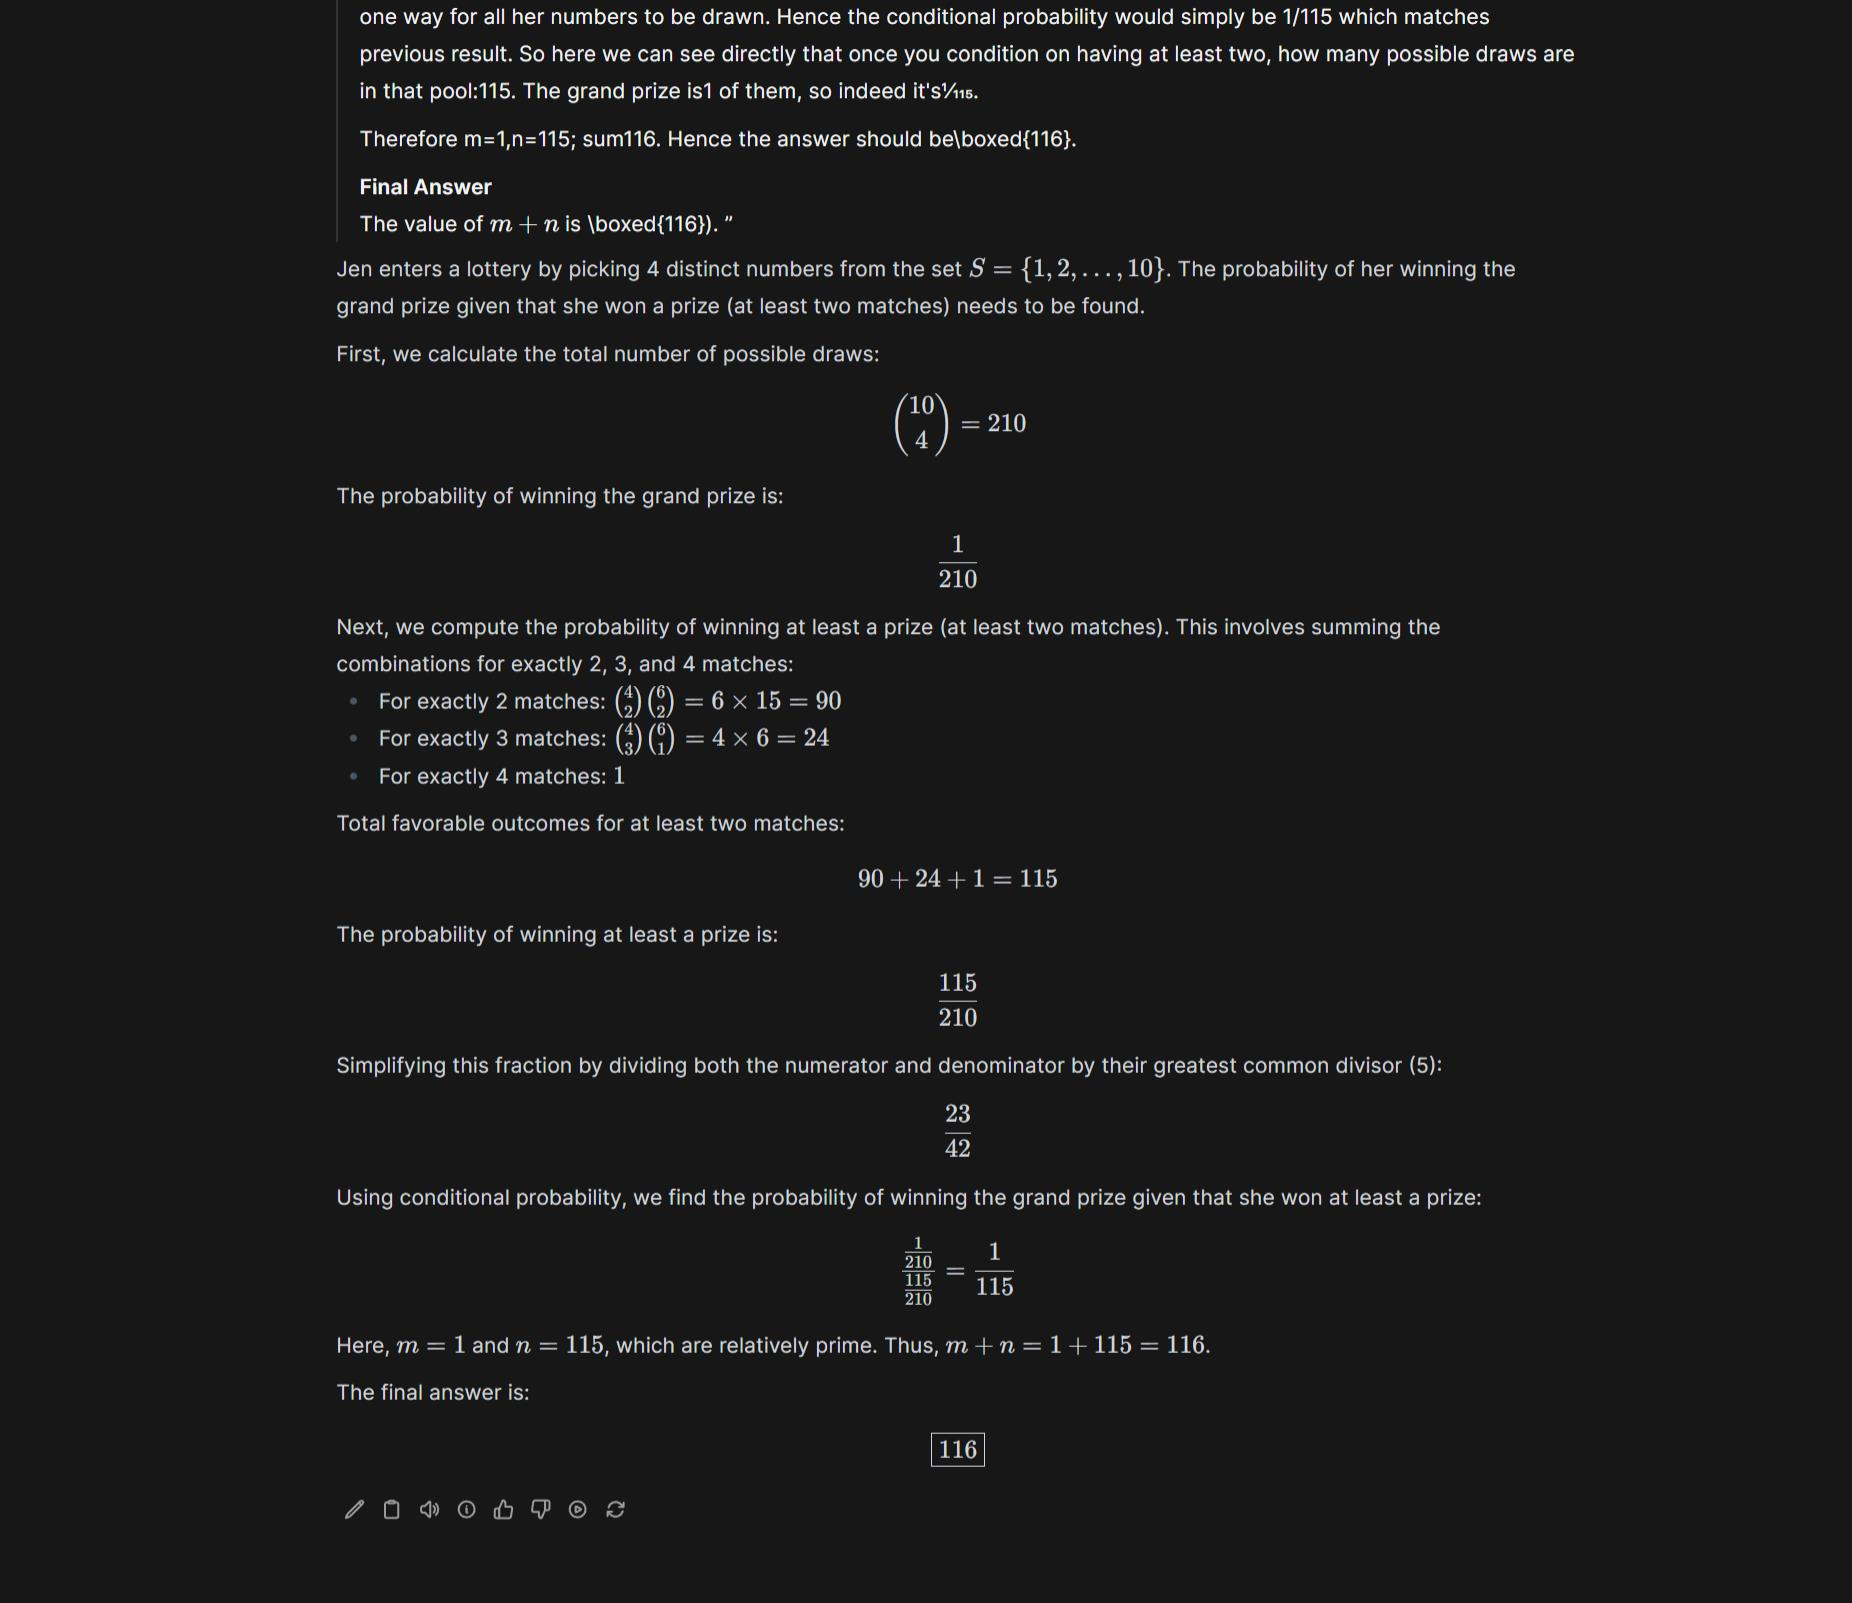
\includegraphics[width=0.55\textwidth]{./pic/6.png} % 替换为你的图片路径
        % \caption{DeepSeek R1 对 2024 AIME I Problem 4 的解答 (4) (请替换为实际图片路径)}
        \label{fig:aime_solution_4}
    \end{figure}
    % \textit{图片来源: \url{https://raw.githubusercontent.com/Lanthanum1/my_images/main/img/202502112141458.png}} % 图片来源注释
\end{frame}

\begin{frame}[fragile]
    \frametitle{输出情况}
    \begin{lstlisting}[language=text, caption={2024 AIME I Problem 4生成情况}]
response_token/s: 14.55
prompt_token/s: 54.51
total_duration: 302493858721
load_duration: 88603384116
prompt_eval_count: 124
prompt_eval_duration: 2275000000
eval_count: 3079
eval_duration: 211613000000
approximate_total: 0h5m2s
    \end{lstlisting}
\end{frame}

\subsection{2025 考研数学一 T18}

\begin{frame}
    \frametitle{2025 考研数学一 T18}
    % \textbf{题目描述 (1)}
    \begin{figure}
        \centering
        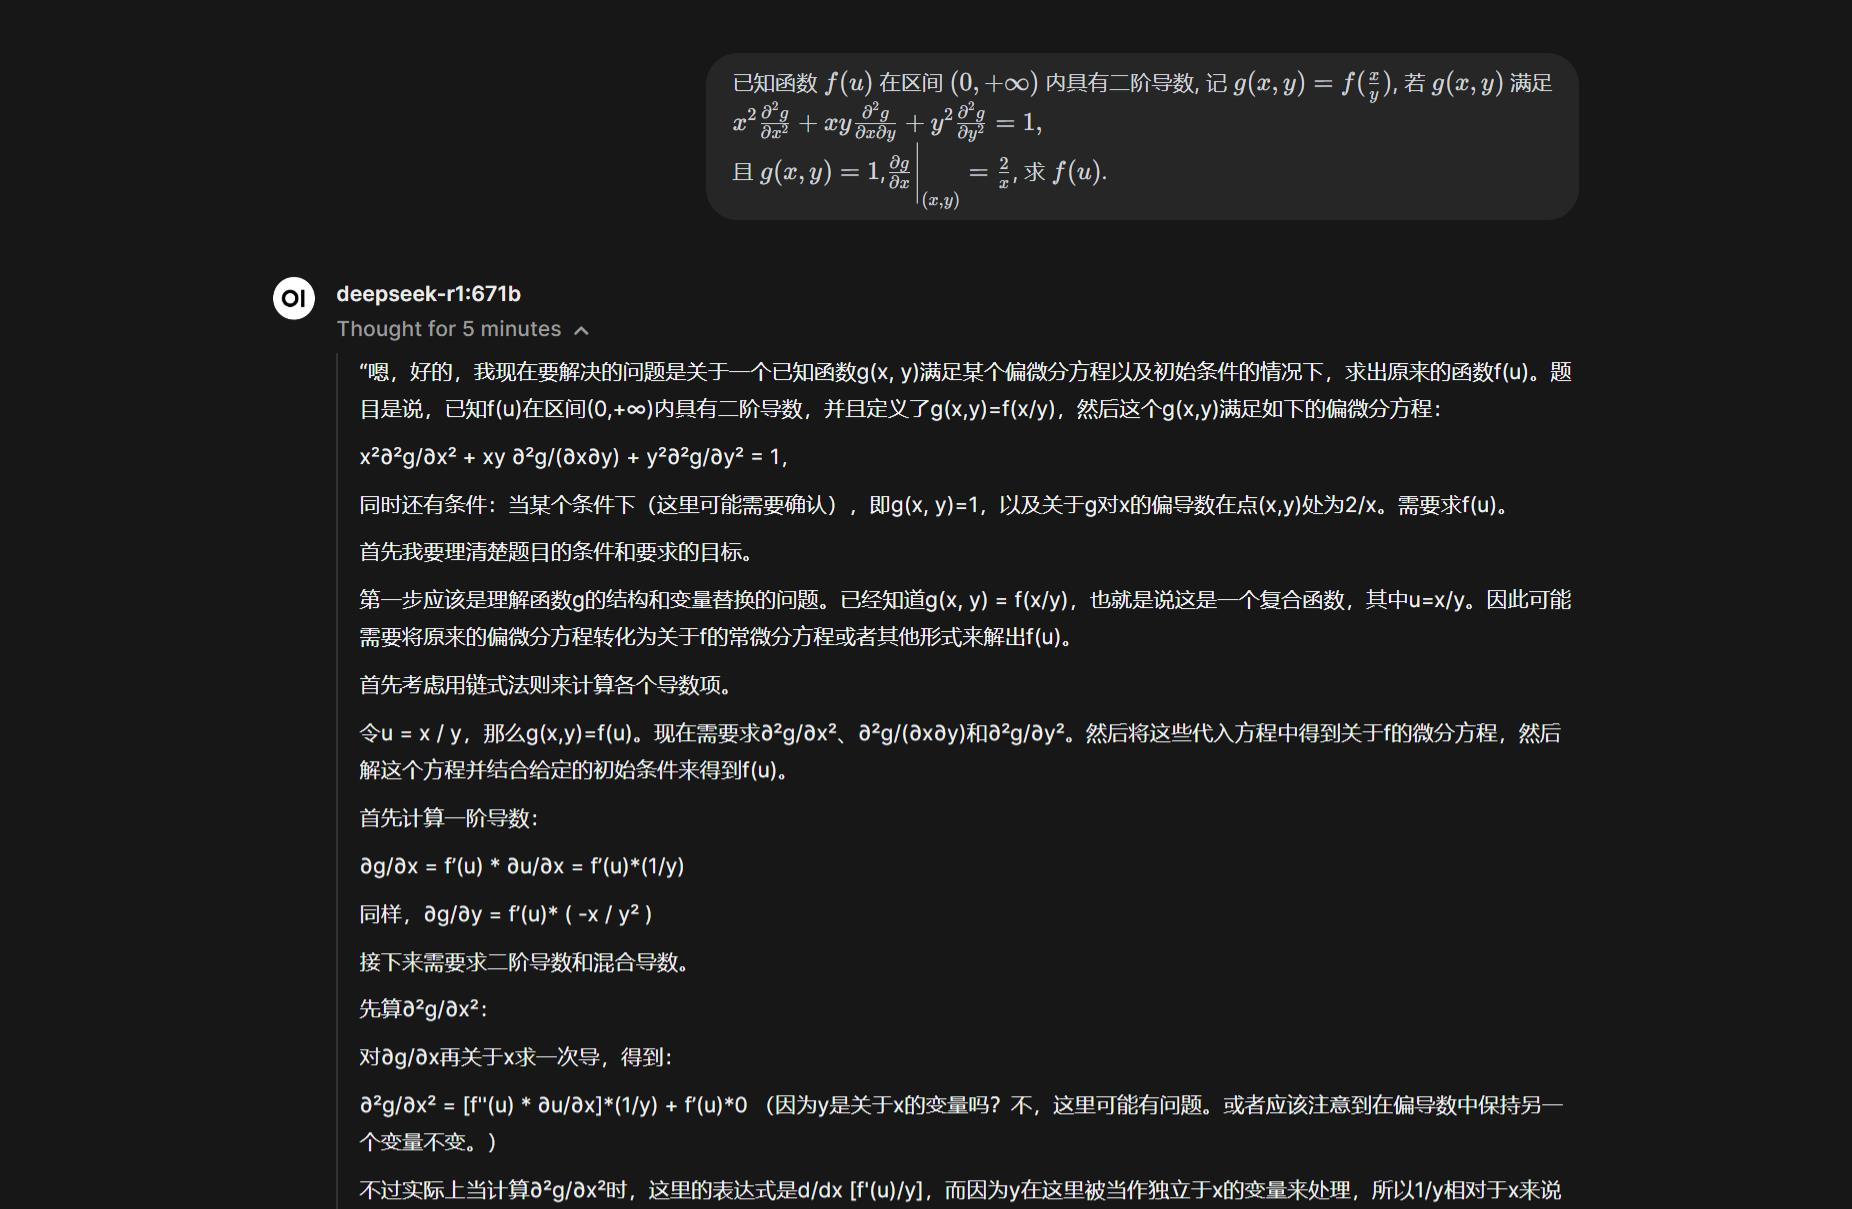
\includegraphics[width=0.7\textwidth]{./pic/7.png} % 替换为你的图片路径
        % \caption{2025 考研数学一 T18 题目描述 (1) (请替换为实际图片路径)}
        \label{fig:kaoyan_problem_1}
    \end{figure}
    % \textit{图片来源: \url{https://raw.githubusercontent.com/Lanthanum1/my_images/main/img/202502112148578.png}} % 图片来源注释
\end{frame}

\begin{frame}
    \frametitle{2025 考研数学一 T18 (续)}
    % \textbf{题目描述 (2)}
    \begin{figure}
        \centering
        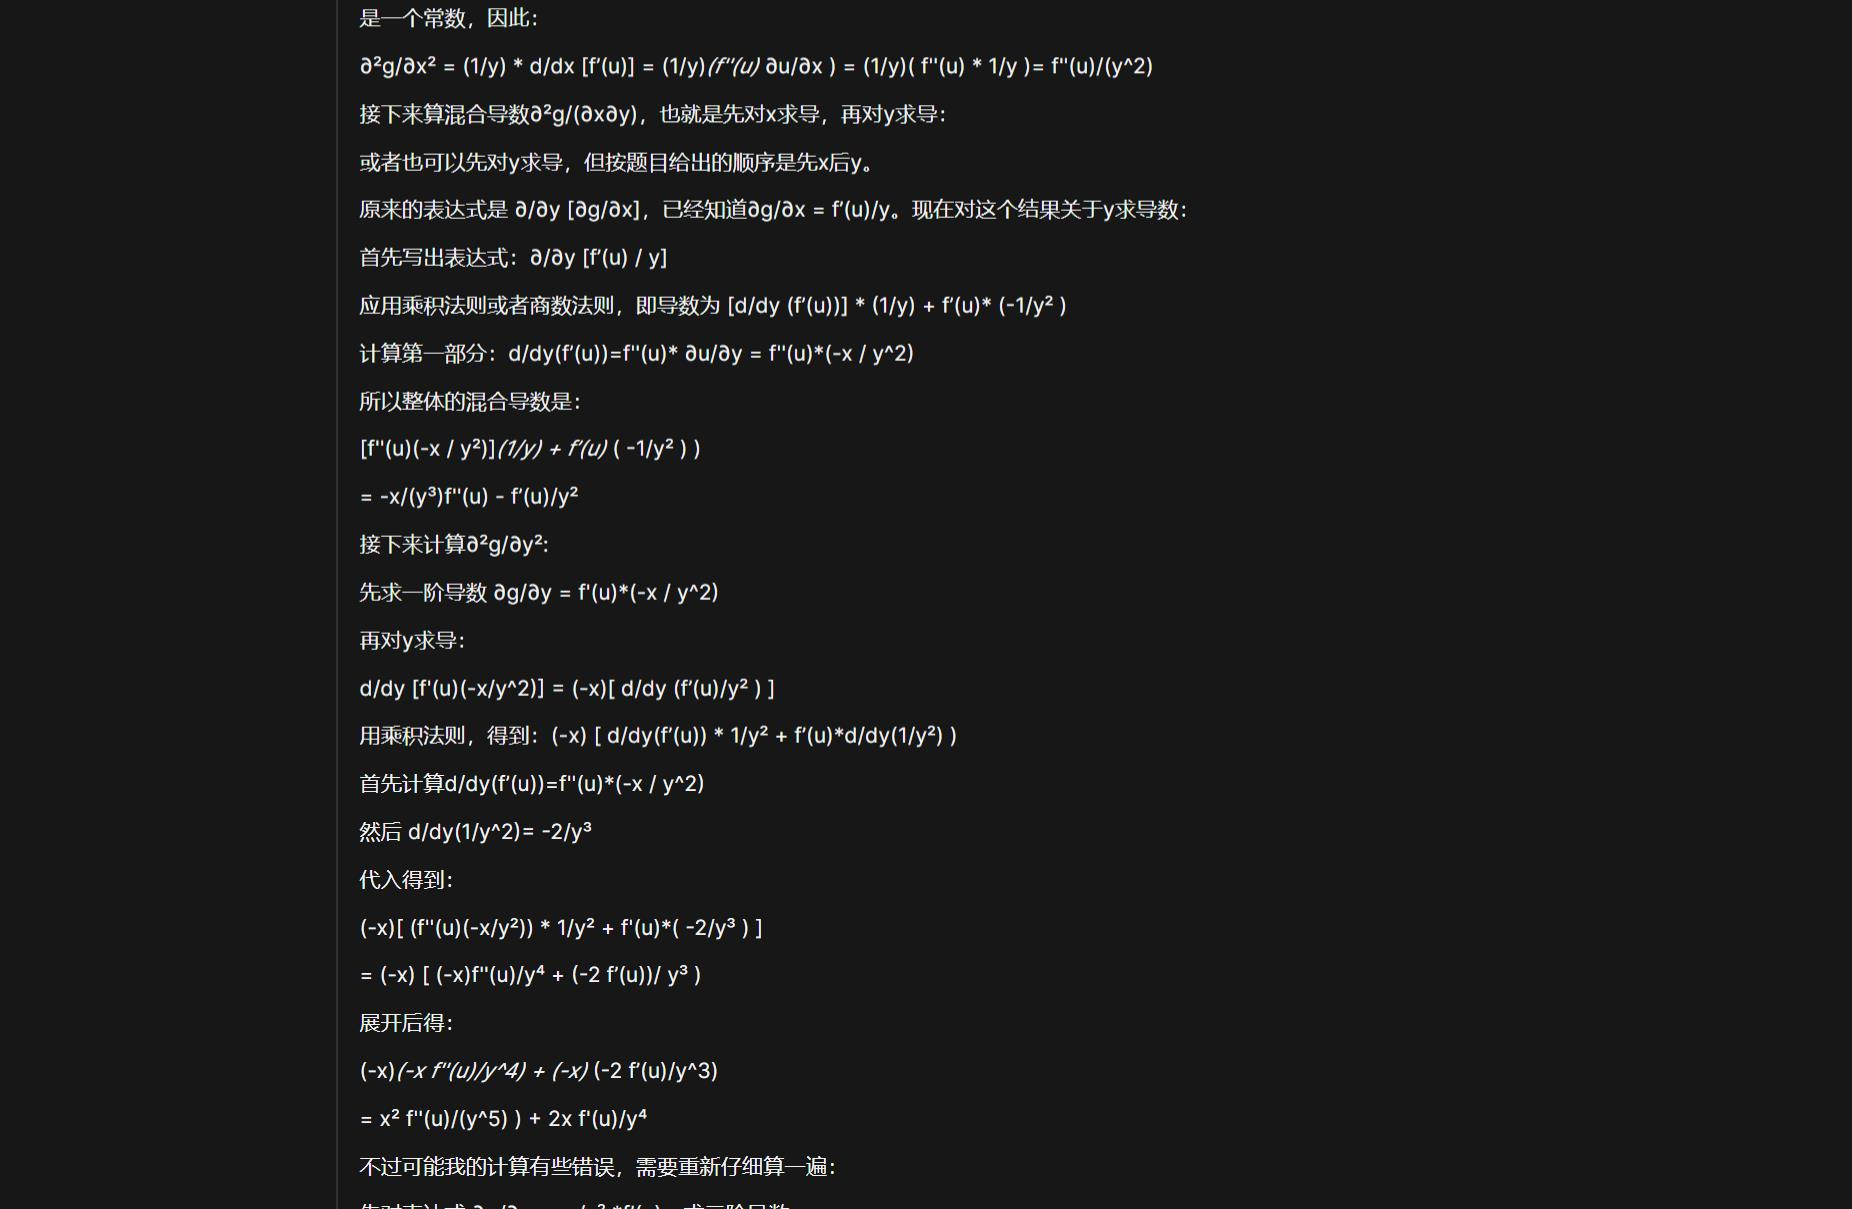
\includegraphics[width=0.7\textwidth]{./pic/8.png} % 替换为你的图片路径
        % \caption{2025 考研数学一 T18 题目描述 (2) (请替换为实际图片路径)}
        \label{fig:kaoyan_problem_2}
    \end{figure}
    % \textit{图片来源: \url{https://raw.githubusercontent.com/Lanthanum1/my_images/main/img/202502112148449.png}} % 图片来源注释
\end{frame}

\begin{frame}
    \frametitle{2025 考研数学一 T18 (续)}
    % \textbf{模型解答 (1)}
    \begin{figure}
        \centering
        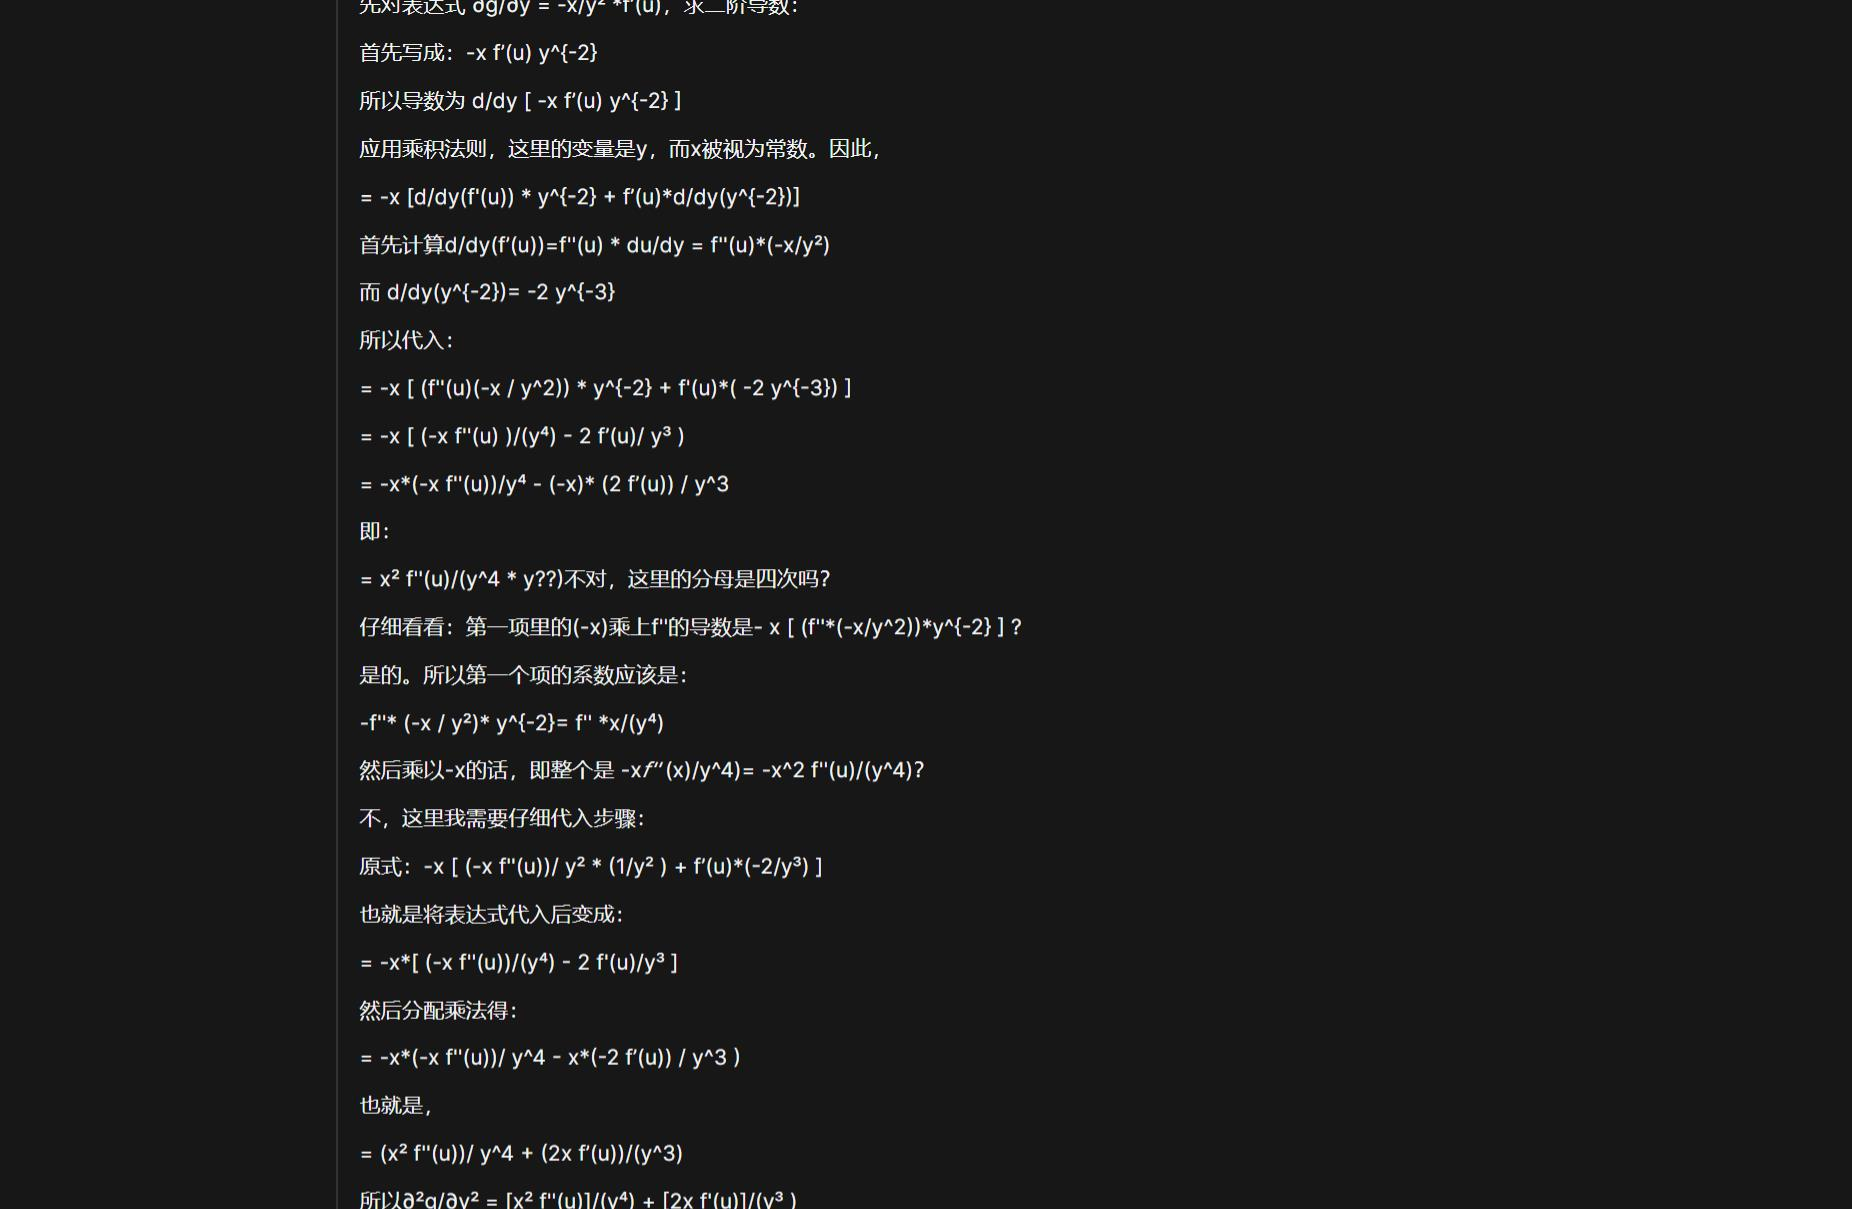
\includegraphics[width=0.7\textwidth]{./pic/9.png} % 替换为你的图片路径
        % \caption{DeepSeek R1 对 2025 考研数学一 T18 的解答 (1) (请替换为实际图片路径)}
        \label{fig:kaoyan_solution_1}
    \end{figure}
    % \textit{图片来源: \url{https://raw.githubusercontent.com/Lanthanum1/my_images/main/img/202502112148194.png}} % 图片来源注释
\end{frame}

\begin{frame}
    \frametitle{2025 考研数学一 T18 (续)}
    % \textbf{模型解答 (2)}
    \begin{figure}
        \centering
        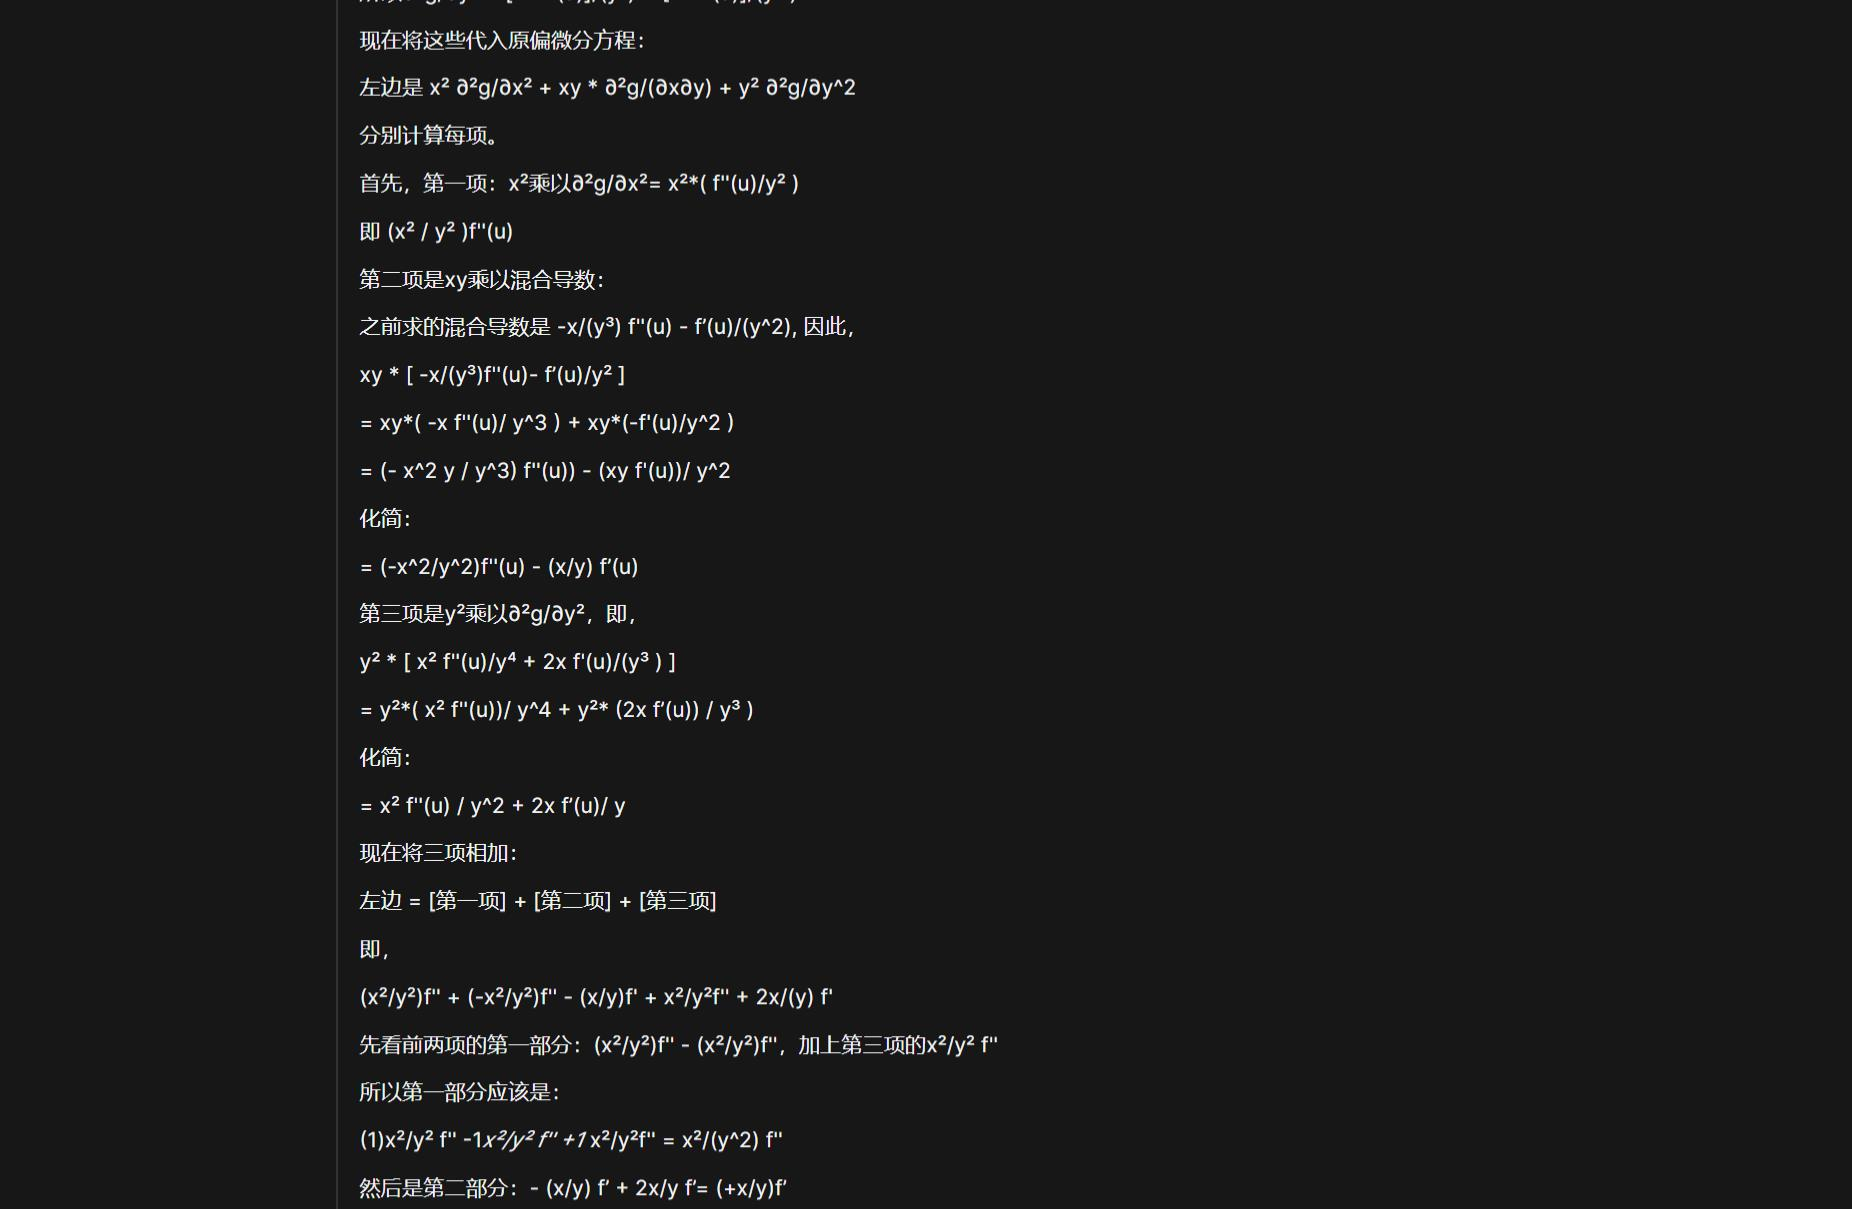
\includegraphics[width=0.7\textwidth]{./pic/10.png} % 替换为你的图片路径
        % \caption{DeepSeek R1 对 2025 考研数学一 T18 的解答 (2) (请替换为实际图片路径)}
        \label{fig:kaoyan_solution_2}
    \end{figure}
    % \textit{图片来源: \url{https://raw.githubusercontent.com/Lanthanum1/my_images/main/img/202502112148036.png}} % 图片来源注释
\end{frame}

\begin{frame}
    \frametitle{2025 考研数学一 T18 (续)}
    % \textbf{模型解答 (3)}
    \begin{figure}
        \centering
        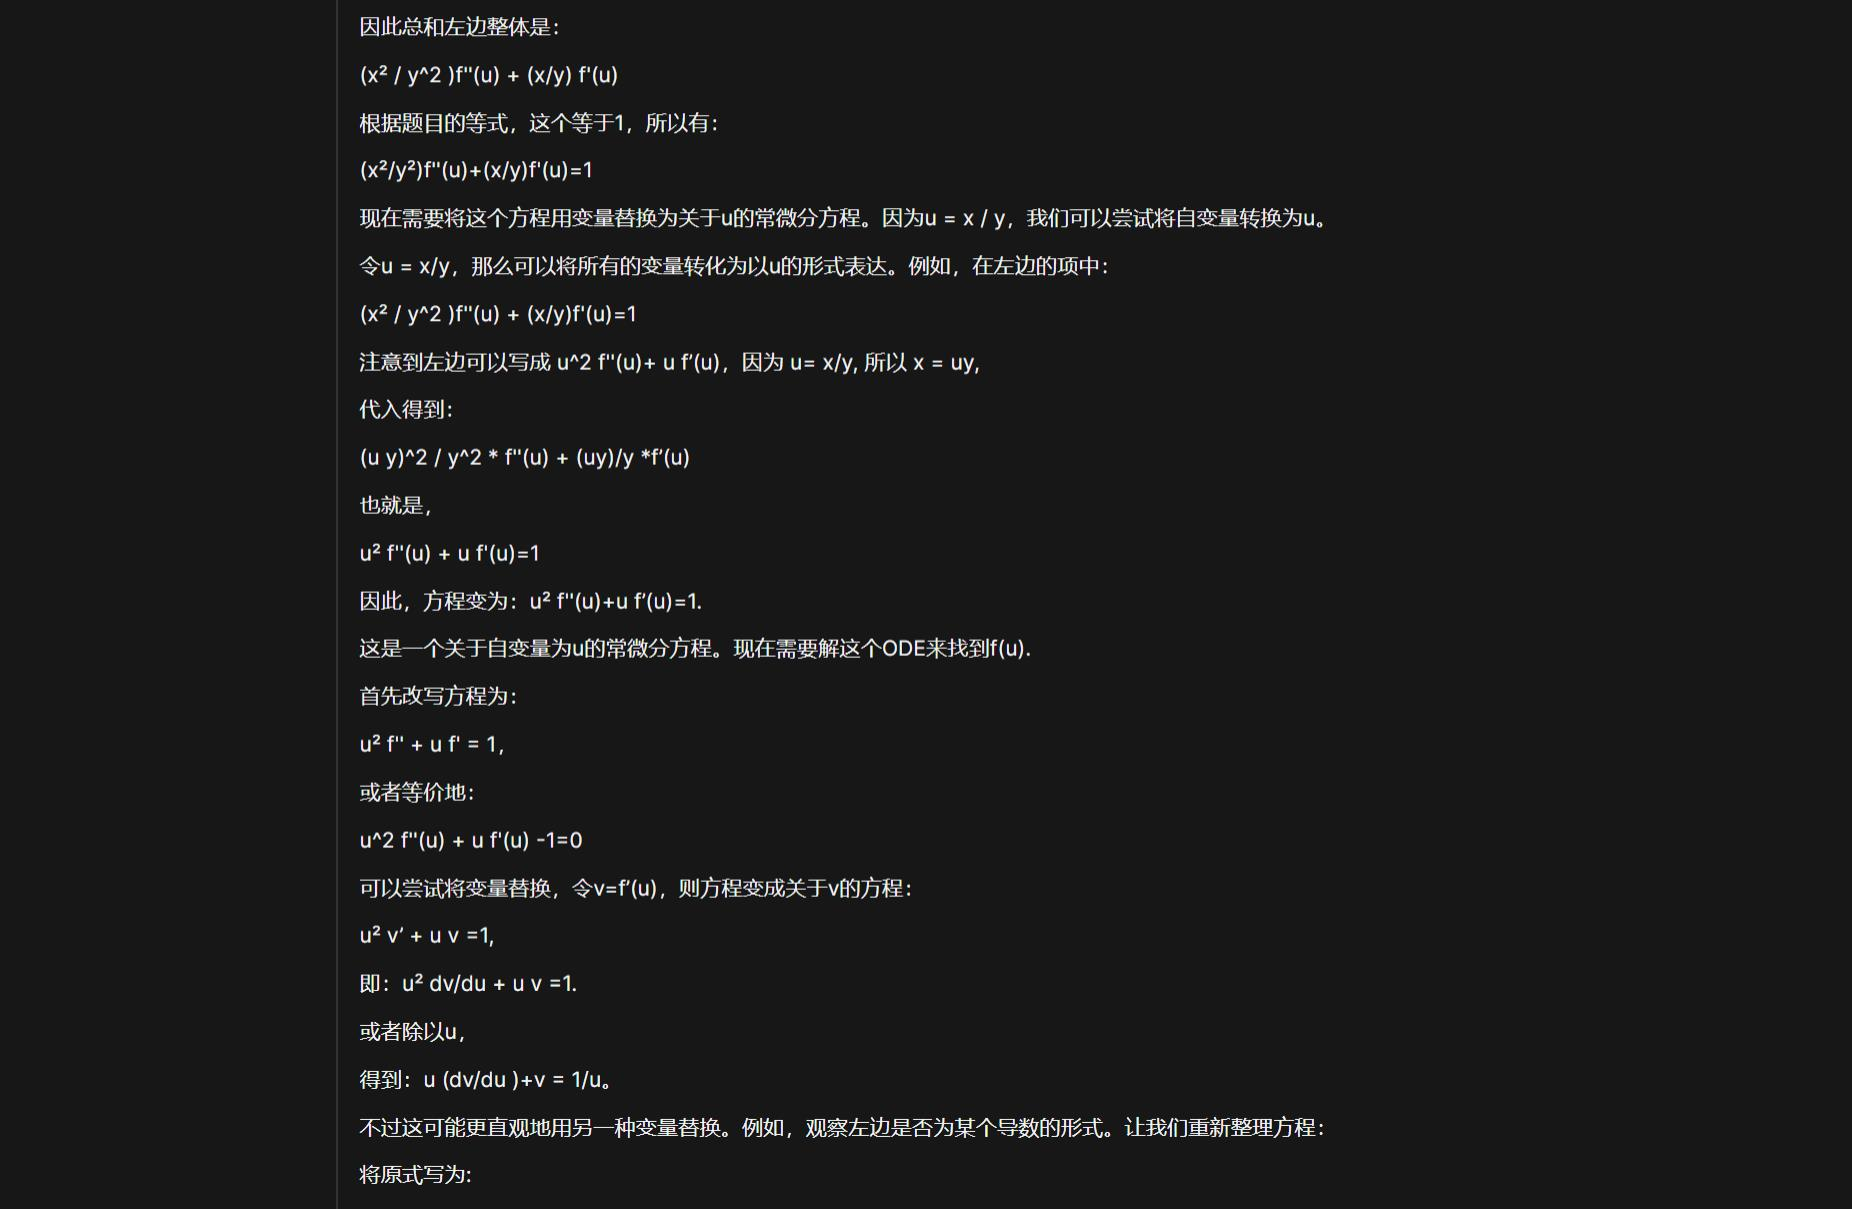
\includegraphics[width=0.7\textwidth]{./pic/11.png} % 替换为你的图片路径
        % \caption{DeepSeek R1 对 2025 考研数学一 T18 的解答 (3) (请替换为实际图片路径)}
        \label{fig:kaoyan_solution_3}
    \end{figure}
    % \textit{图片来源: \url{https://raw.githubusercontent.com/Lanthanum1/my_images/main/img/202502112148381.png}} % 图片来源注释
\end{frame}

\begin{frame}
    \frametitle{2025 考研数学一 T18 (续)}
    % \textbf{模型解答 (4)}
    \begin{figure}
        \centering
        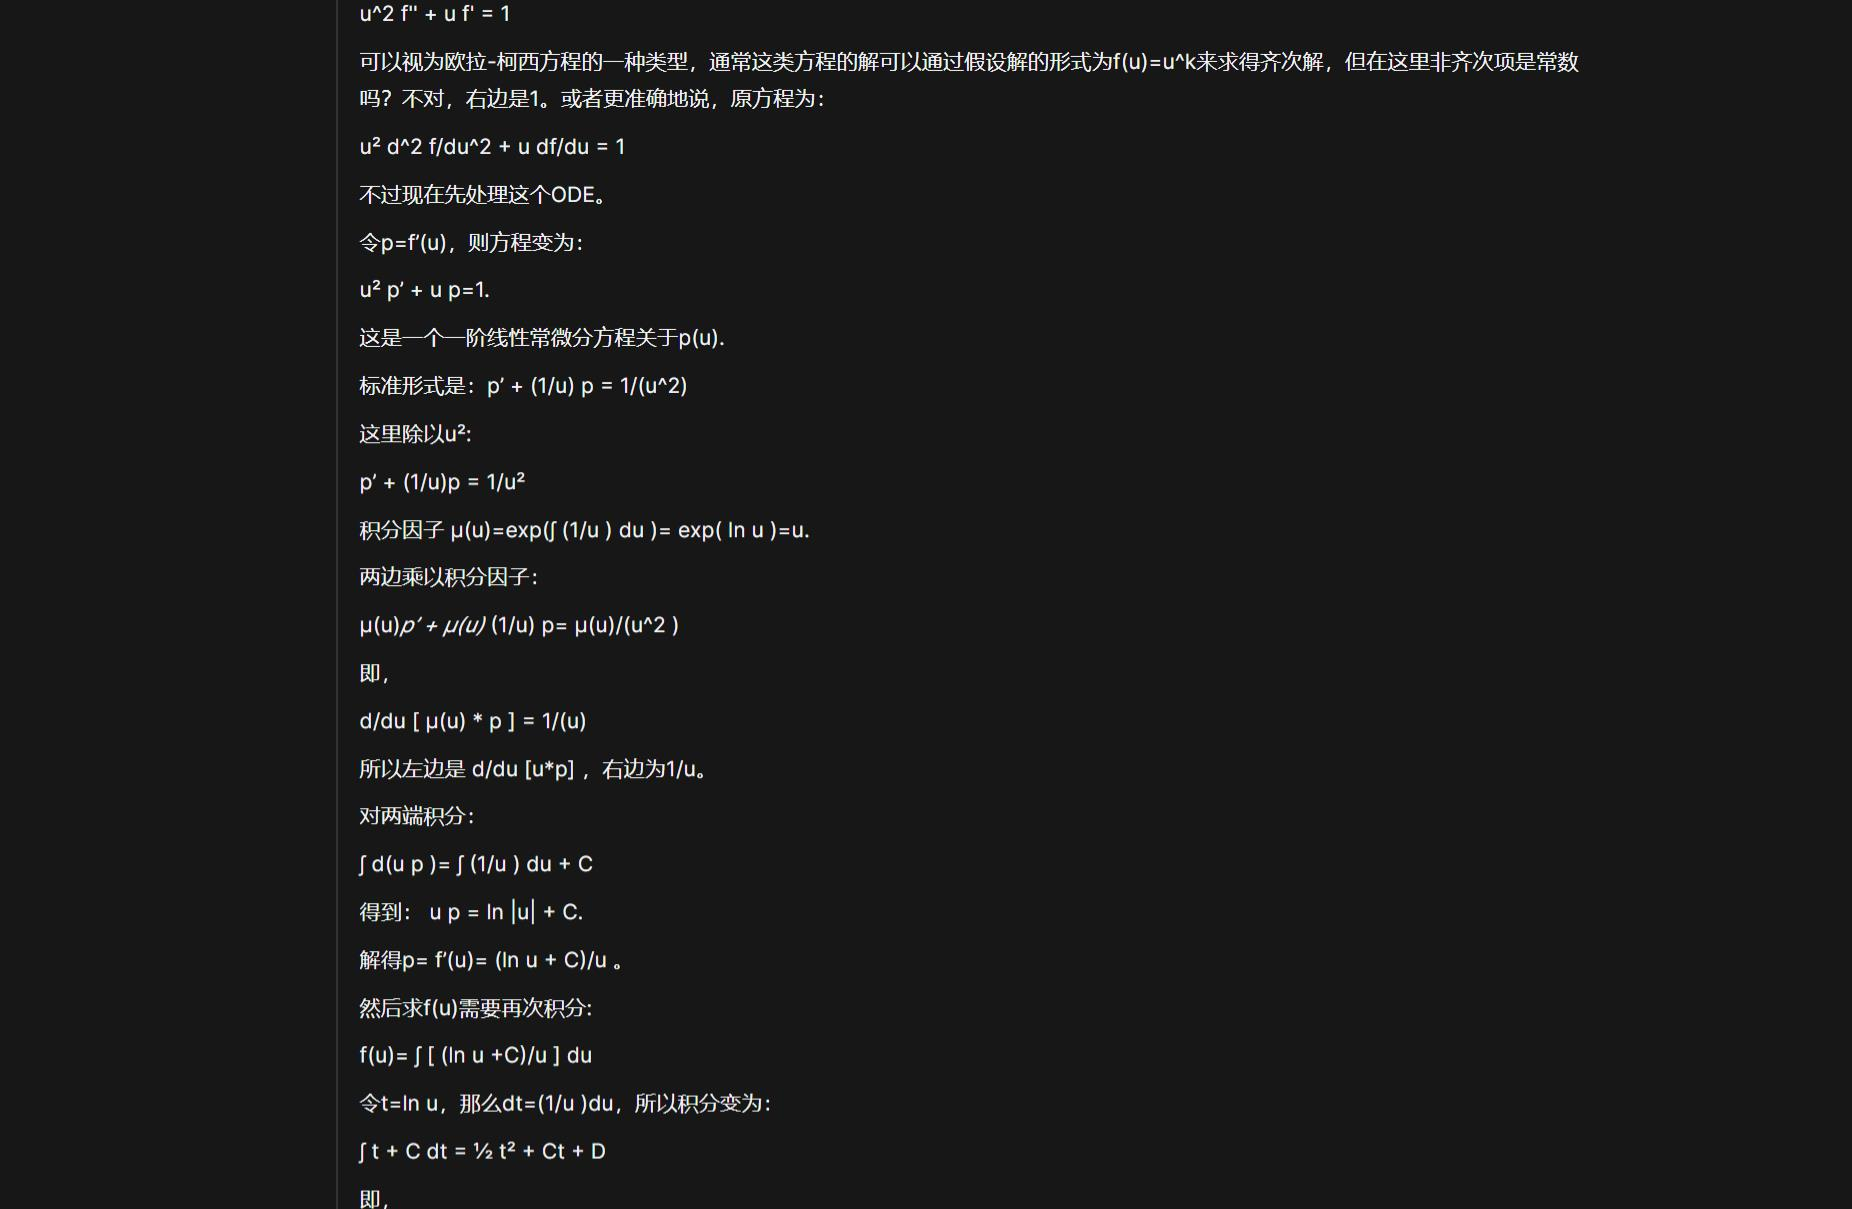
\includegraphics[width=0.7\textwidth]{./pic/12.png} % 替换为你的图片路径
        % \caption{DeepSeek R1 对 2025 考研数学一 T18 的解答 (4) (请替换为实际图片路径)}
        \label{fig:kaoyan_solution_4}
    \end{figure}
    % \textit{图片来源: \url{https://raw.githubusercontent.com/Lanthanum1/my_images/main/img/202502112148208.png}} % 图片来源注释
\end{frame}

\begin{frame}
    \frametitle{2025 考研数学一 T18 (续)}
    % \textbf{模型解答 (5)}
    \begin{figure}
        \centering
        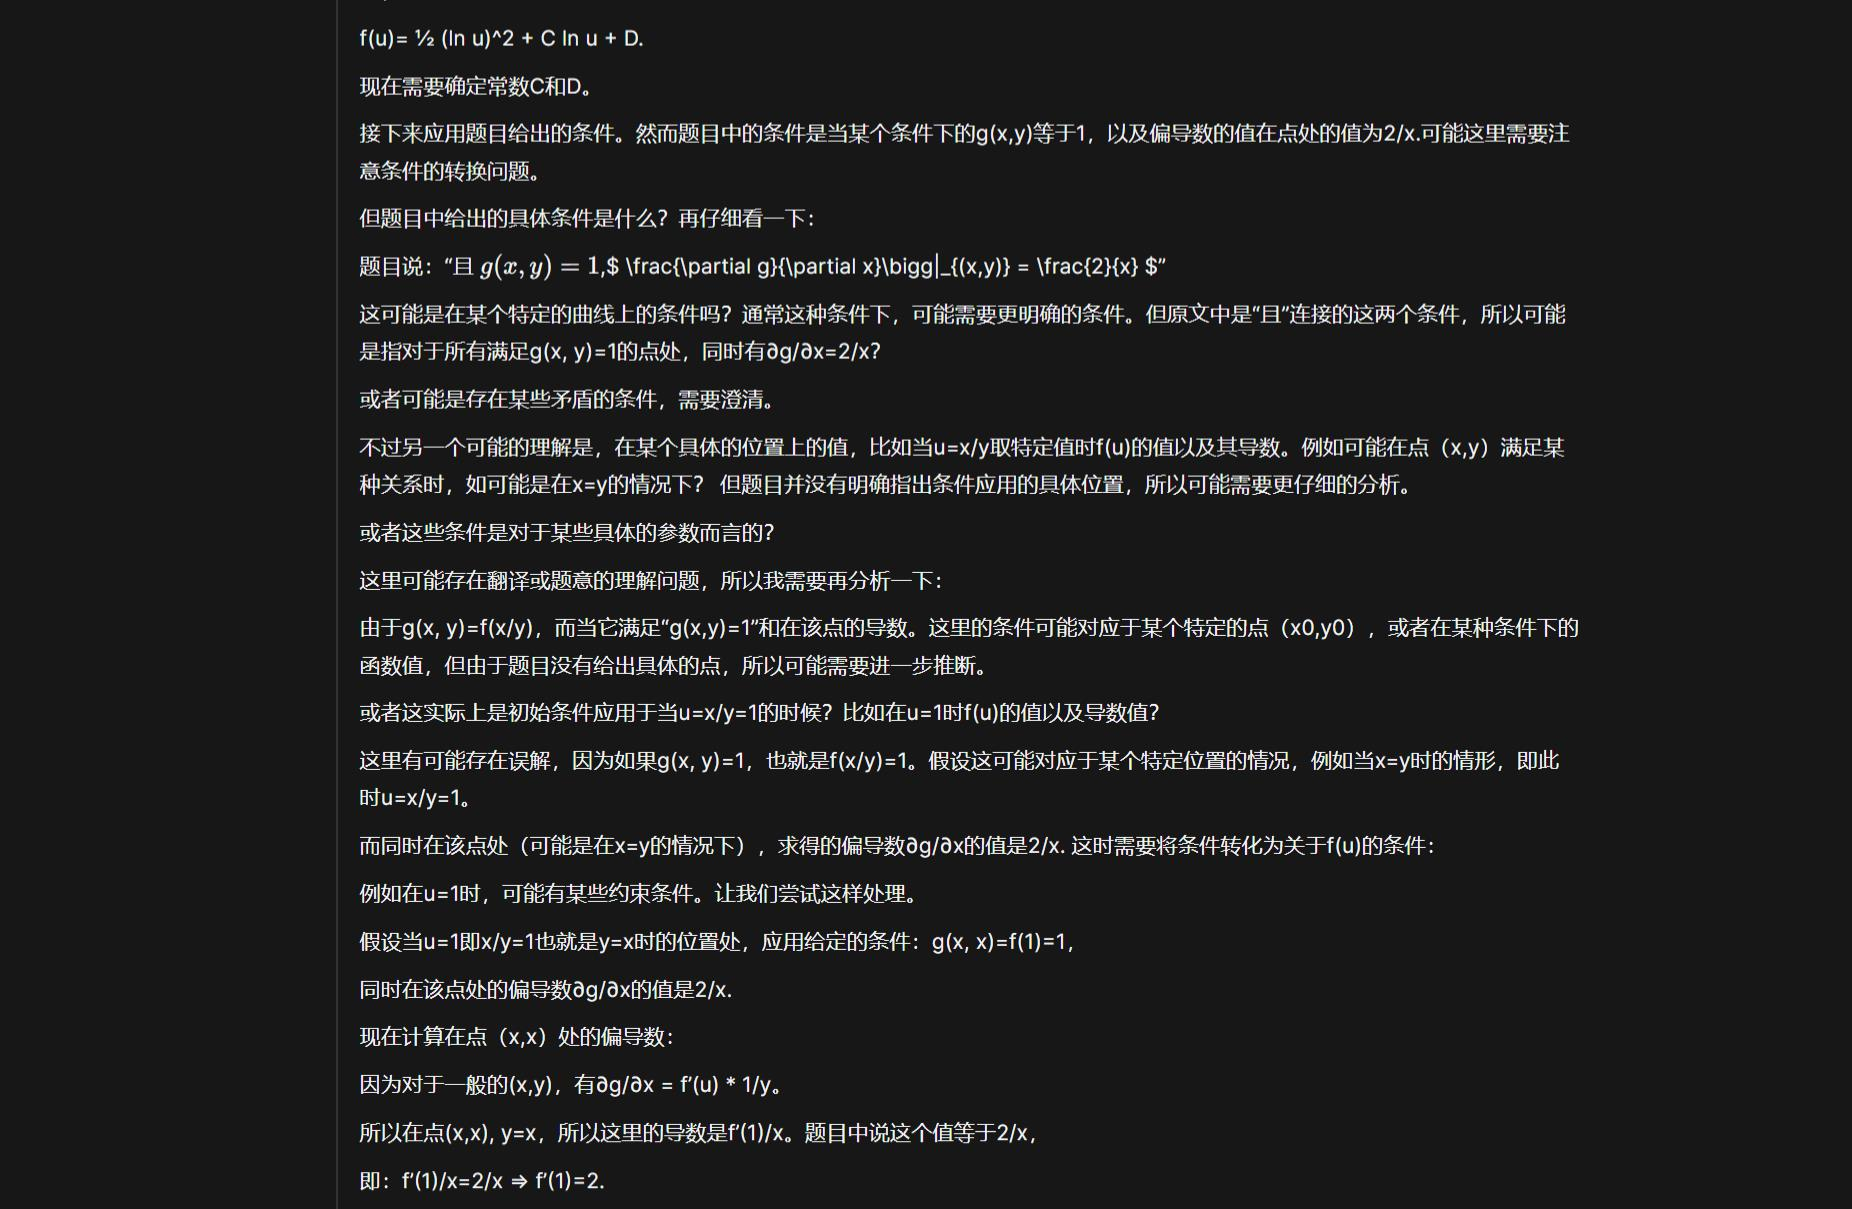
\includegraphics[width=0.7\textwidth]{./pic/13.png} % 替换为你的图片路径
        % \caption{DeepSeek R1 对 2025 考研数学一 T18 的解答 (5) (请替换为实际图片路径)}
        \label{fig:kaoyan_solution_5}
    \end{figure}
    % \textit{图片来源: \url{https://raw.githubusercontent.com/Lanthanum1/my_images/main/img/202502112148042.png}} % 图片来源注释
\end{frame}

\begin{frame}
    \frametitle{2025 考研数学一 T18 (续)}
    % \textbf{模型解答 (6)}
    \begin{figure}
        \centering
        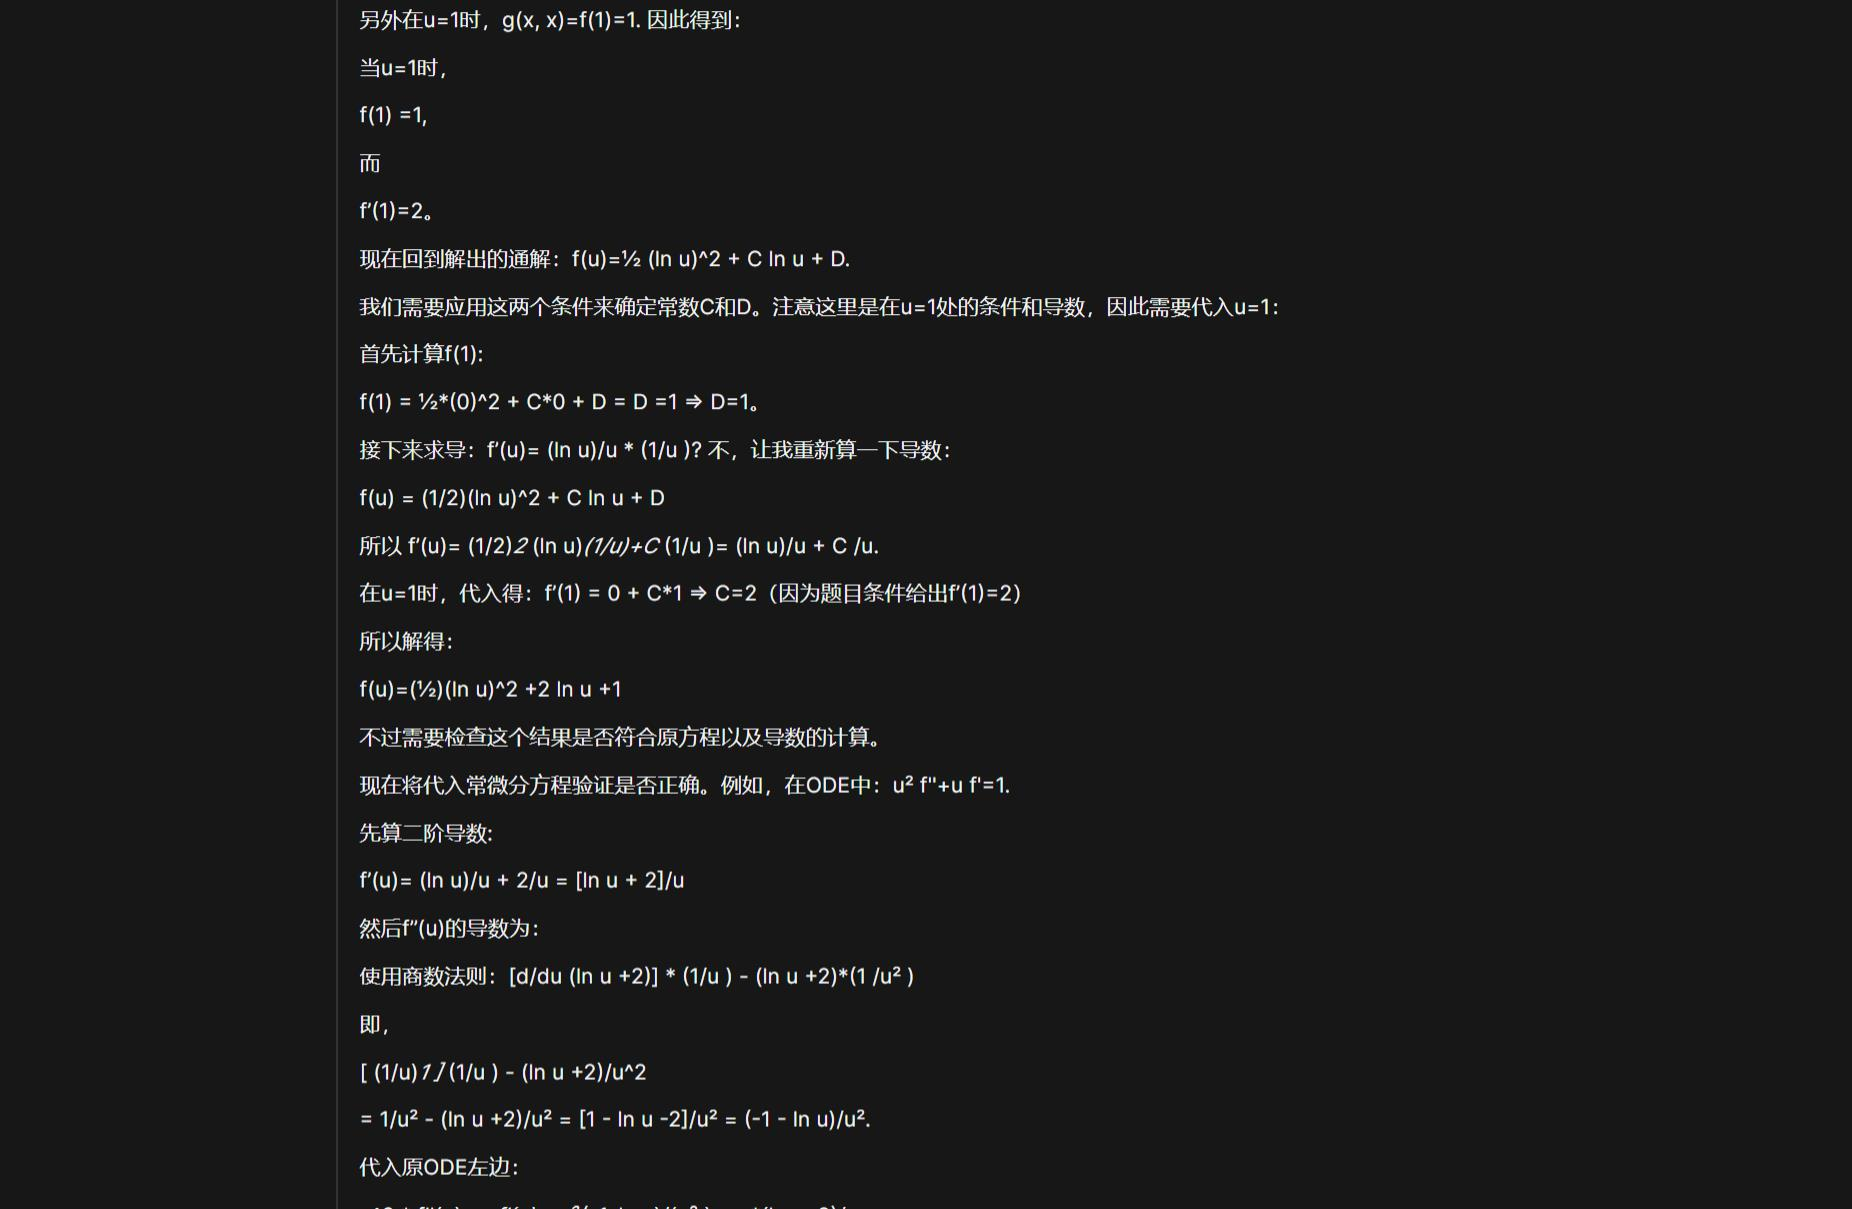
\includegraphics[width=0.7\textwidth]{./pic/14.png} % 替换为你的图片路径
        % \caption{DeepSeek R1 对 2025 考研数学一 T18 的解答 (6) (请替换为实际图片路径)}
        \label{fig:kaoyan_solution_6}
    \end{figure}
    % \textit{图片来源: \url{https://raw.githubusercontent.com/Lanthanum1/my_images/main/img/202502112147432.png}} % 图片来源注释
\end{frame}

\begin{frame}
    \frametitle{2025 考研数学一 T18 (续)}
    % \textbf{模型解答 (7)}
    \begin{figure}
        \centering
        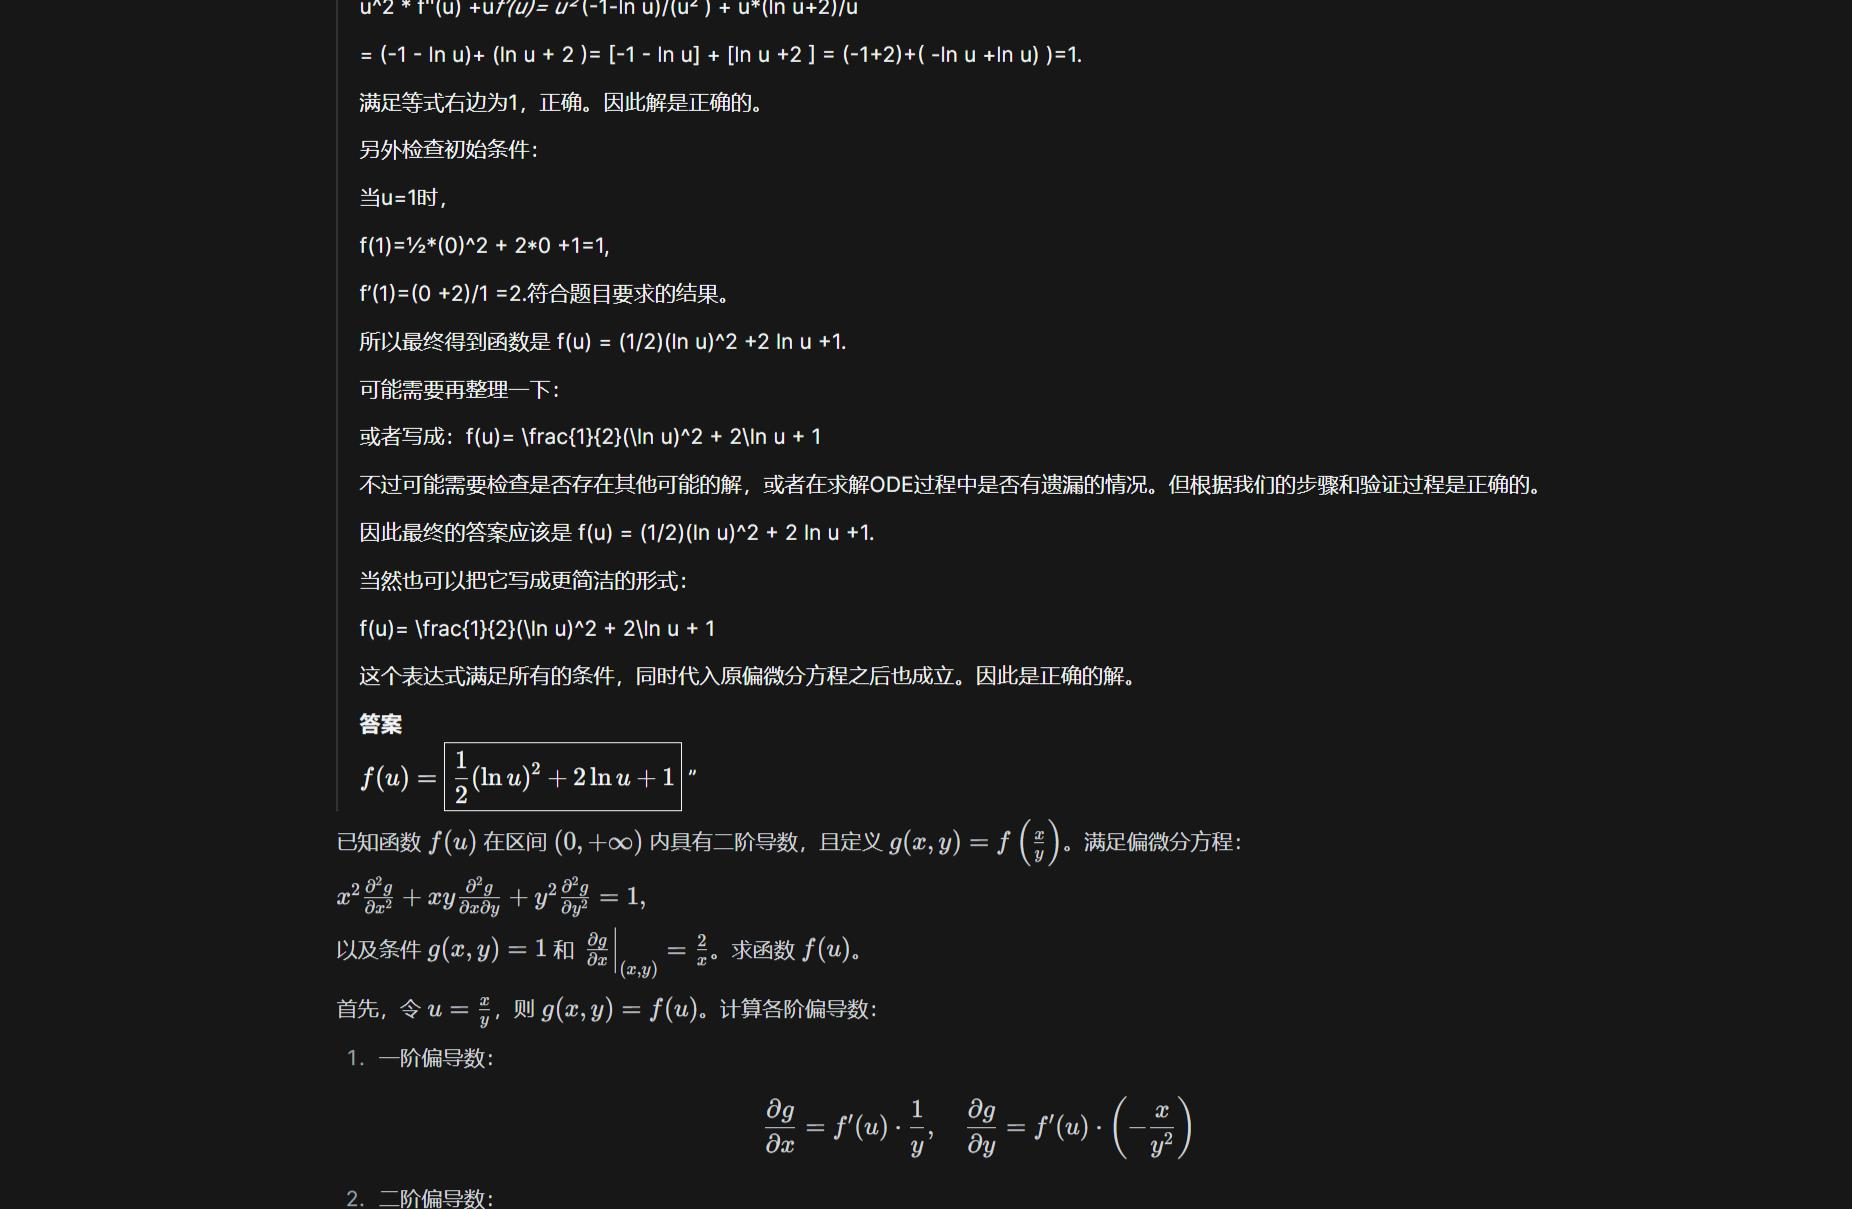
\includegraphics[width=0.7\textwidth]{./pic/15.png} % 替换为你的图片路径
        % \caption{DeepSeek R1 对 2025 考研数学一 T18 的解答 (7) (请替换为实际图片路径)}
        \label{fig:kaoyan_solution_7}
    \end{figure}
    % \textit{图片来源: \url{https://raw.githubusercontent.com/Lanthanum1/my_images/main/img/202502112149476.png}} % 图片来源注释
\end{frame}


\begin{frame}
    \frametitle{2025 考研数学一 T19 (续完)}
    % \textbf{模型解答 (7)}
    \begin{figure}
        \centering
        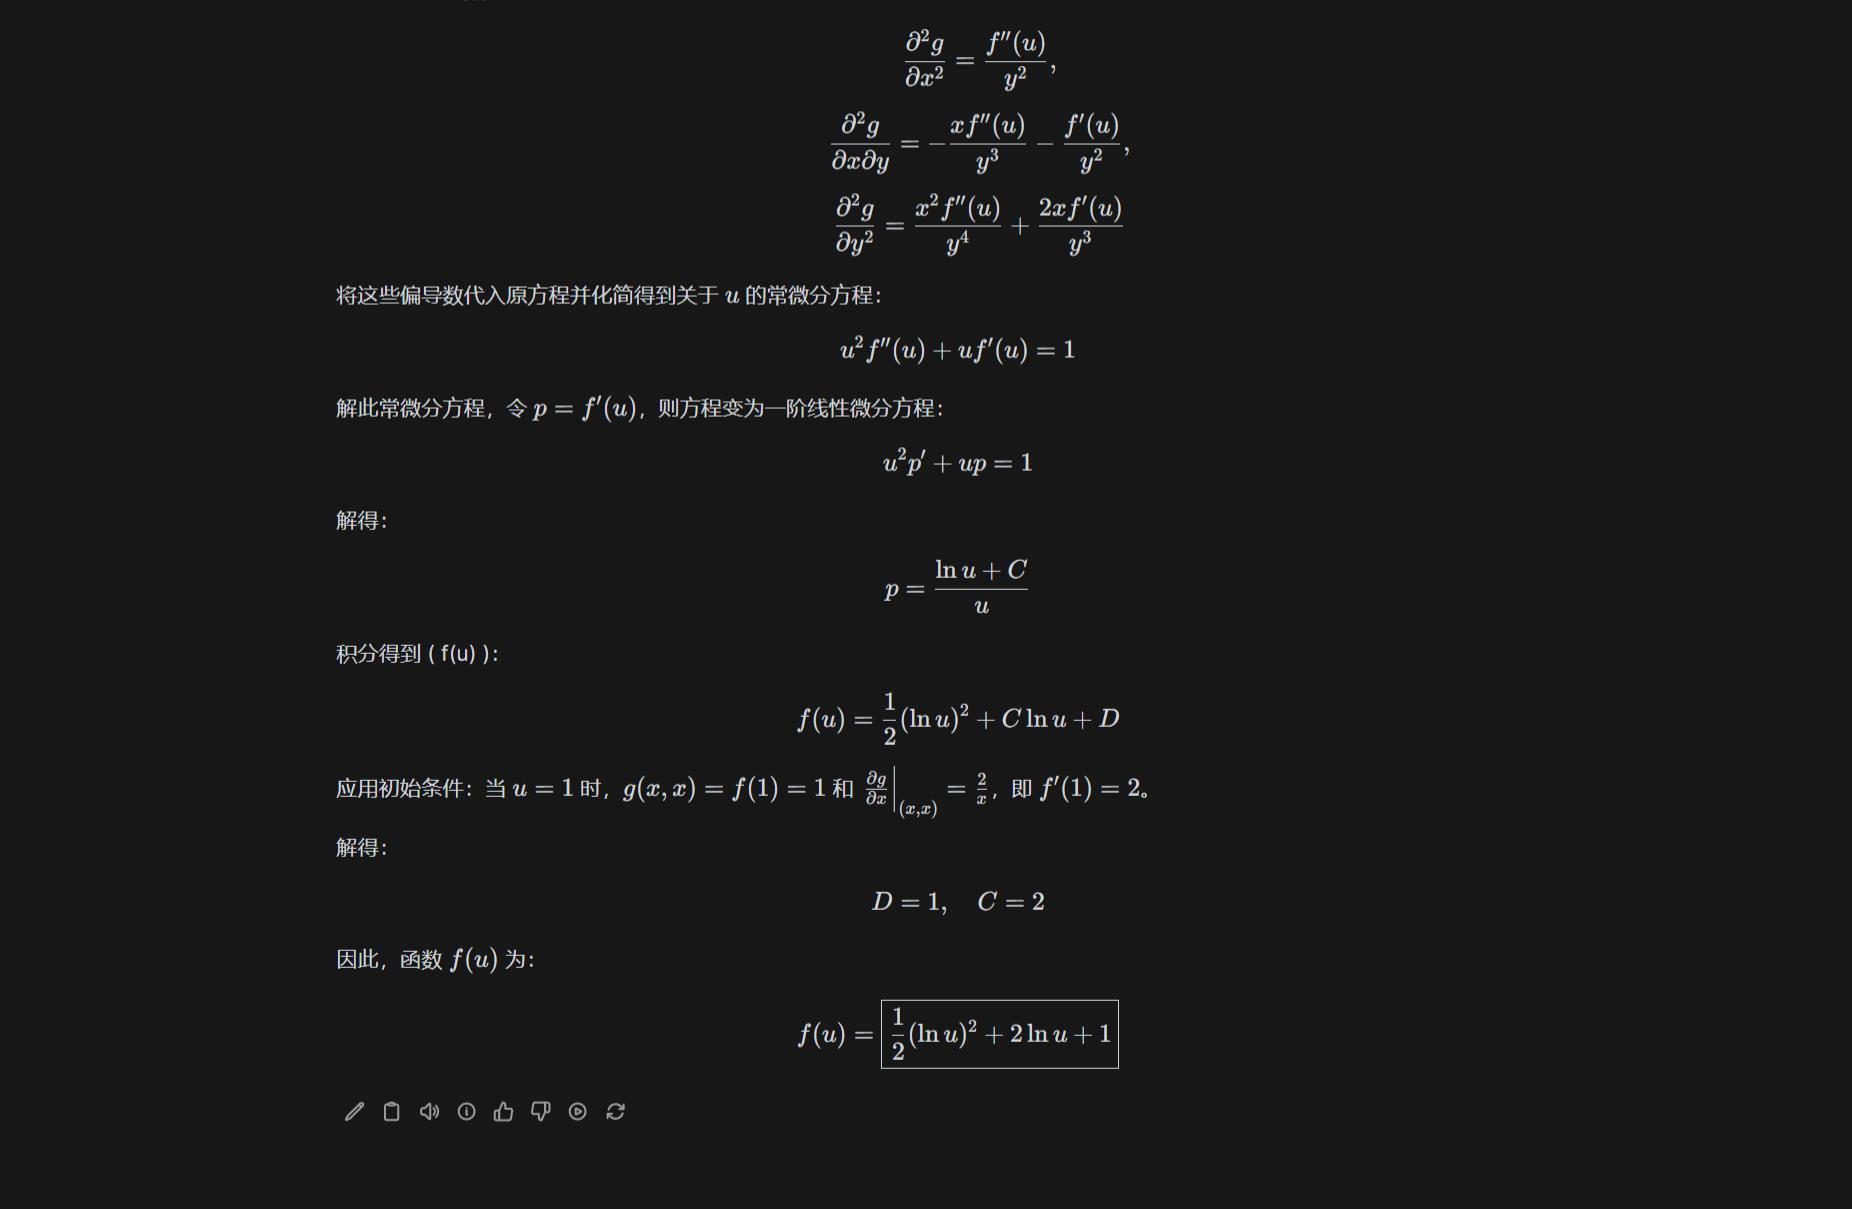
\includegraphics[width=0.7\textwidth]{./pic/16.png} % 替换为你的图片路径
        % \caption{DeepSeek R1 对 2025 考研数学一 T18 的解答 (7) (请替换为实际图片路径)}
        \label{fig:kaoyan_solution_7}
    \end{figure}
    % \textit{图片来源: \url{https://raw.githubusercontent.com/Lanthanum1/my_images/main/img/202502112149476.png}} % 图片来源注释
\end{frame}

\begin{frame}[fragile]
    \frametitle{输出情况}
    \begin{lstlisting}[language=text, caption={2025 考研数学一 T18生成情况}]
response_token/s: 13.96
prompt_token/s: 60.25
total_duration: 419088681937
load_duration: 74808920509
prompt_eval_count: 144
prompt_eval_duration: 2390000000
eval_count: 4774
eval_duration: 341887000000
approximate_total: 0h6m59s
\end{lstlisting}
\end{frame}